\documentclass[a4paper,oneside,12pt]{book}
%----------------------------------------------------------------------------------------
%	WELCOME!
%   It's probably worth having a read through this file to set up the broad parameters.
%----------------------------------------------------------------------------------------

%----------------------------------------------------------------------------------------
%	COVER PAGE
%   The cover page is laid out in title/title.tex. You can choose a colour
%   or black and white logo
%----------------------------------------------------------------------------------------

%----------------------------------------------------------------------------------------
%	THESIS INFORMATION
%   Put title, author name, degree, type of work, school, department in here
%   It will be used for the title page and for the embedded PDF information
%----------------------------------------------------------------------------------------

\newcommand{\thesistitle}{Federated Meta-Learning: A Novel Approach for Algorithm Selection} % Your thesis title, this is used in the title and abstract
\newcommand{\degree}{Master of Science in Computer Science (Data Science)} % Your degree name, this is used in the title page and abstract
\newcommand{\typeofthesis}{Dissertations} % dissertation, Final Year Project, report, etc.
\newcommand{\authorname}{Mukesh Arambakam} % Your name, this is used in the title page and PDF stuff
%% Comment out the next line if you don't want your ID to appear
\newcommand{\authorid}{19301497} % Your ID
\newcommand{\keywords}{Federated Meta Learning, Meta Learning, Algorithm Selection, ...} % Keywords for your thesis
\newcommand{\school}{\href{http://www.scss.tcd.ie}{School of Computer Science and Statistics}} % Your school's name and URL, this is used in the title page

%% Comment out the next line if you don't want a department to appear
%\newcommand{\department}{\href{http://researchgroup.university.com}{Department Name}} % Your research group's name and URL, this is used in the title page

\AtBeginDocument{
\hypersetup{pdftitle=\thesistitle} % Set the PDF's title to your title
\hypersetup{pdfauthor=\authorname} % Set the PDF's author to your name
\hypersetup{pdfkeywords=\keywords} % Set the PDF's keywords to your keywords
\hypersetup{pdfsubject=\degree} % Set the PDF's keywords to your keywords
}

%% Language and font encodings
\usepackage[T1]{fontenc} 
\usepackage[utf8]{inputenc}
\usepackage[english]{babel}

%% Bibliographical stuff
\usepackage[round,sort,comma,numbers]{natbib}

%% Document size
% include showframe as an option if you want to see the boxes
\usepackage[a4paper,top=2.54cm,bottom=2.54cm,left=2.54cm,right=2.54cm,headheight=16pt]{geometry}

%% Useful packages
\usepackage{amsmath}
\usepackage[autostyle=true]{csquotes} % Required to generate language-dependent quotes in the bibliography
\usepackage[pdftex]{graphicx}
\usepackage[colorinlistoftodos]{todonotes}
\usepackage[colorlinks=true, allcolors=black]{hyperref}
\usepackage{caption} % if no caption, no colon
\usepackage{sfmath} %use sans-serif in the maths sections too
\usepackage[parfill]{parskip}    % Begin paragraphs with an empty line rather than an indent
\usepackage{setspace} % to permit one-and-a-half or double spacing
\usepackage{enumerate} % fancy enumerations like (i) (ii) or (a) (b) and suchlike
\usepackage{booktabs} % To thicken table lines
\usepackage{fancyhdr}
\usepackage{float}

\usepackage{listings}
\usepackage{color}
\usepackage{ragged2e}
\usepackage{caption}
\usepackage{subcaption}

\pagestyle{plain} % Embrace simplicity!

%% Code Highlighting
\definecolor{dkgreen}{rgb}{0,0.6,0}
\definecolor{gray}{rgb}{0.5,0.5,0.5}
\definecolor{mauve}{rgb}{0.58,0,0.82}

\lstset{frame=tb,
  language=Python,
  aboveskip=3mm,
  belowskip=3mm,
  showstringspaces=false,
  columns=flexible,
  basicstyle={\small\ttfamily},
  numbers=none,
  numberstyle=\tiny\color{gray},
  keywordstyle=\color{blue},
  commentstyle=\color{dkgreen},
  stringstyle=\color{mauve},
  breaklines=true,
  breakatwhitespace=true,
  tabsize=3
}


%% The Mechanical engineers require your name and ID on the top of every page.
%% Uncomment the following block if you want your name and ID at the top of
%% (almost) every page.

%\pagestyle{fancy}
%\fancyhf{} % sets both header and footer to nothing
%\renewcommand{\headrulewidth}{0pt}
%\cfoot{\thepage}
%\ifdefined\authorid
%\chead{\it \authorname\ (\authorid)}
%\else
%\chead{\it \authorname}
%\fi
%% End of block

%% It is not a requirement of the university that the font should be sans-serif, but
%% the Mechanical engineers require it. Comment out the following line to disable it
\renewcommand{\familydefault}{\sfdefault} %use the sans-serif font as default

%% If you're not using sans-serif, consider using Palatino instead of the LaTeX standard
%\usepackage{mathpazo} % Use the Palatino font by default if you prefer it to Computer Modern

\renewcommand{\theequation}{\arabic{equation}} %% use continuous equation numbers

%% Format Chapter headings appropriately
\usepackage{titlesec}
\titleformat{\chapter}[hang] 
{\normalfont\huge\bfseries}{\thechapter}{1cm}{} 

\title{\thesistitle}
\author{\authorname}

\frontmatter
\begin{document}
\begin{titlepage}

\center % Center everything on the page

%% All the text parameters should be taken from the start of the main.tex file.
%% You should only alter stuff here if you want to change the layout

%----------------------------------------------------------------------------------------
%	LOGO SECTION
%----------------------------------------------------------------------------------------
%% Choose one of the following -- a colour or black-and-white logo


\includegraphics{title/Trinity_RGB_transparent_main.png}\\[1cm] 
%
\includegraphics[width=12cm]{title/black-stacked-trinity.jpg}\\[1cm] 

\Large \school\\[1.5cm] % Minor heading such as course title
\ifdefined\department
\large \department\\[1.5cm] % Minor heading such as course title
\fi

%----------------------------------------------------------------------------------------
%	TITLE SECTION
%----------------------------------------------------------------------------------------
\makeatletter
{ \huge \bfseries \thesistitle}\\[1.5cm] % Title of your document
 

%----------------------------------------------------------------------------------------
%	AUTHOR SECTION
%----------------------------------------------------------------------------------------

\ifdefined\authorid
\authorname\\ % Your name
\authorid\\[2cm] % Your Student ID
\else
\authorname\\[2cm] % Your name
\fi

%----------------------------------------------------------------------------------------
%	DATE SECTION
%----------------------------------------------------------------------------------------

{\large \today}\\[2cm] % Date, change the \today to a set date if you want to be precise

 
%----------------------------------------------------------------------------------------
%	TYPE OF THESIS SECTION
%----------------------------------------------------------------------------------------
 A \typeofthesis\ submitted in partial fulfilment\\of the requirements for the degree of\\
\degree

\vfill % Fill the rest of the page with whitespace

\end{titlepage}


%%%
%%% Set up page layout parameters.
%%%
\setlength\paperheight{297mm}
\setlength\paperwidth{210mm}

\setlength{\textheight}{235mm} %{8in}- 1/4"        BKay
\setlength{\oddsidemargin}{10mm}  %{0.5in} + 1/8" BKay
\setlength{\evensidemargin}{10mm} %{0.5in}        BKay
\setlength{\textwidth}{155mm}
%\setlength{\topmargin}{0.62in} %{0.5in}+1/8"        BKay
%\setlength{\headheight}{0in}
%\setlength{\headsep}{0in}
%\setlength{\parindent}{12mm}


\pagenumbering{roman}

%% DECLARATION %%
\section*{\Huge{Declaration}}
\vspace{1cm}
I hereby declare that the work described in this dissertation is, except where otherwise stated, entirely my own work, and has not been submitted as an exercise for a degree at this or any other university

\vspace{1cm}
I have read and I understand the plagiarism provisions in the General Regulations of the University Calendar for the current year, found at \url{http://www.tcd.ie/calendar}.
\vspace{1cm}

I have also completed the Online Tutorial on avoiding plagiarism `Ready Steady Write', located at
\url{http://tcd-ie.libguides.com/plagiarism/ready-steady-write}.
\vspace{3cm}

Signed:~\rule{5cm}{0.3pt}\hfill Date:~\rule{5cm}{0.3pt}
\newpage

%% LEND LIBRARY %%
\section*{\Huge{Permission to lend and/or copy}}
\vspace{1cm}
I agree that the Trinity College Library may lend or copy this dissertation upon request.

\vspace{3cm}

Signed:~\rule{5cm}{0.3pt}\hfill Date:~\rule{5cm}{0.3pt}


\newpage


\onehalfspacing\raggedright %\raggedright turns off justification and hypenation

\section*{\Huge{Acknowledgements}}
Throughout the course of this dissertation I have received a great deal of support and assistance from a lot of people.

First and foremost, I would like to thank my supervisor, Dr. Joeran Beel, for the research idea and for his continuous support throughout the project. I also would like to thank him for believing in me and giving me the autonomy to work on the project and develop each stage of the application as I wanted.

Secondly, I would like thank my friends Manasi, Aishwarya and Jagadish, who provided me with advice and proof read my report. I would also like to thank them for their efforts in acting as alpha testers of the application and providing me with valuable feedback in improving the user-experience of the application.

Finally, I would like to thank my family for their constant support and patience during these unforeseen circumstances, especially my mother for her constant moral support without whom this would not have been possible. Thanks Mum!

\singlespacing\justify
\chapter*{Abstract}
\quad\quad “Federated Meta-Learning” (FML), a concept that allows everyone to benefit from the data that is generated through software libraries including machine learning and data science libraries. It focuses on learning the algorithm performance measures and making recommendations based on the model created. I introduce FMLearn, an application developed using the client-server model, which allows the exchange of meta-data about machine learning models and data in itself, for the purpose of meta-learned algorithm selection and configuration. 
The input to FMLearn is a dataset and the output is a recommendation for the potentially best performing algorithm(s) and it’s hyper-parameters to solve the task. This recommendation is made by a model built using the Meta-Features obtained from the dataset description, using the K-Nearest Neighbours algorithm and historic performance data.
Scikit-Learn’s toy datasets along with other datasets from UCI Machine Learning repository were used and evaluated against various machine learning algorithms using GridSearchCV and Cross-Validation for which the execution time was measured.
In the case previously seen datasets like scikit-learn’s breast cancer dataset, an execution time of approximately 94.24min was recorded to find the best algorithm by performing Grid Search and Cross-Validation. Whereas, when FMLearn was asked to recommend the best algorithm, the application only took 3secs to recommend the best performing algorithm along with its model parameters.
For a large dataset like the skin segmentation, traditional means for finding the best performing algorithms takes approximately 869.74 minutes and when FMLearn was asked to recommend the same, it took only 3secs.
In the case of previously unseen but similar datasets, the recommended algorithm is accurate, but the hyper-parameters required re-optimisation to suite the dataset. For a previously unseen and highly dissimilar dataset, FMLearn recommends a list of algorithms which it thinks are best suited for that dataset based on its prior knowledge. In this case, FMLearn recommends the best performing algorithm about 60\% of the time.
Overall, the use of this application allows the user to scale down an average of 86.718\% and 95.762\% of time and electricity for small and large datasets respectively by eliminating the repetitive and time consuming task of algorithm selection and configuration from the Machine Learning Workflow. 

\subsection*{Keywords}
{Federated Meta-Learning, FMLearn, AutoML, Machine Learning, RecSys, Dataset Meta-Features, Algorithm Selection, Algorithm Configuration}

%%A short summary of the problem investigated, the approach taken and the key findings. This should be around 400 words, or less.

%%This should be on a separate page.

\onehalfspacing\raggedright %\raggedright turns off justification and hypenation
\newpage

\tableofcontents
\listoffigures
\listoftables
\newpage
\section*{\Huge{Nomenclature}}
\begin{tabular}{lp{9cm}l}
Auto*&Automated\\
AutoML&Automated Machine Learning\\
API&Application Programming Interface\\
DAA&Distributed Application Architecture\\
FML&Federated Meta-Learning\\
HTTP&Hypertext Transfer Protocol\\
JSON&JavaScript Object Notation\\
KNN&K-Nearest Neighbours\\
ML&Machine Learning\\
MtL&Meta-Learning\\
NF&Normal Form\\
NP& Non-Deterministic Polynomial Time\\
PaaS&Platform as a Service\\
SAT&propositional satisfiability problem\\
SQL&Structured Query Language\\
SVM&Support Vector Machines\\

${\displaystyle{i}}$&Single Instance from a Set\\
${\displaystyle{m}}$&Cost Metric\\
${\displaystyle{\mathcal{A}}}$&Algorithm\\
${\displaystyle{\mathcal{D}}}$&Dataset\\
${\displaystyle{\mathcal{I}}}$&Set of Instances\\
${\displaystyle{\mathcal{P}}}$&Portfolio of Algorithms\\
${\displaystyle{\mathcal{R}}}$&Problem Statement

\end{tabular}
\vspace{2cm}

All measurements of time used in the report are in \textbf{minutes} unless specified otherwise.

All measurements of power specified in this report are in \textbf{watts} unless specified otherwise.


\justify
\mainmatter
\chapter{Introduction}
An ever-growing number of algorithms are used to solve machine learning and data science tasks and the challenge of algorithm selection and configuration is subject to intensive research.  \citep{bischl-et-al,brazdil:p,calandra-et-al,collins-et-al2018,romero-et-al,vartak-et-al}. 

    %%\textbf{expand on this research in sec2?} 

Meta-learning is one of the most promising techniques to warm starting the algorithm selection and configuration process - \citep{hutter-et-al}. With meta-learning, a machine learning model is trained to predict how algorithms perform on a given task. The meta-learning model is built based on the past performance of algorithms on a large number of tasks or datasets, which are described through meta-features. For unseen tasks, the best performing algorithms can be predicted through the meta-learner (and subsequently be optimized with e.g. Bayesian Hyper-Parameter Optimization).

\section{Motivation}
A challenge in algorithm selection and configuration is the (non) availability of data in some disciplines to build the meta-learning model, which is due to the workflow of machine learning, data science or other projects. Typically, software libraries – be it machine learning libraries like Auto-sklearn \citep{feurer:m}, Auto-Weka \citep{kotthoff:l} or ML-Plan \citep{mohr:f}, recommender system libraries like LibRec-Auto \citep{mansoury:m}, are used in isolation, either locally or in the cloud. By “in isolation” I mean that the information regarding how algorithms perform on a particular dataset, is neither published nor shared. Consequently, computationally expensive algorithm selection and hyper parameter optimization is performed by each machine learning engineer over and over again for the same datasets, which is a huge waste of Time, Electricity, Computational Power and Money.

\section{Background}
The task of Algorithm Selection is usually done on an instance by instance basis. There are many tools which offer this feature like Auto-Sklearn, OpenML, etc., but these tools select the best performing algorithm by predicting the performance of each algorithm for a given task by running various algorithms on a subset of the entire dataset and then choosing the best performing algorithm on that subset for the task. Though this is just a over-simplified explanation of what the libraries do internally, this is a task that takes up a lot of time, electricity and computational power before it could suggest the best suited algorithm for the task. Even if the task is to find the best algorithm for a previously seen dataset the entire process is repeated.

The same can be said for Hyper-Parameter Optimisation / Tuning as well, this is a process of selecting a set of optimal hyper-parameters for an algorithm. A hyper-parameter is a parameter whose value is used control how a machine learning algorithm solves a given problem. Hyper-Parameter Optimisation is also a task that takes a great deal of time, electricity and computational power, before a optimal set of hyper-parameter can be chosen for an algorithm-dataset pair.

\section{Research Problem}
The time, electricity, computational power and money spent for the task of algorithm selection and hyper-parameter optimisation is justifiable for the first time search for the best algorithm is done. But, with the increasing popularity and use of Machine Learning for various tasks, time, electricity and computational power spent for finding the best algorithm for a given a dataset, along with it's optimal hyper-parameters becomes a repetitive task.

The problem here is the workflow of machine learning and data science libraries, these libraries usually work in isolation and the information regarding how an algorithm performs on a particular dataset is neither publisher nor shared. Which leads to computationally expensive and time consuming task like algorithm selection and hyper-parameter optimisation being performed over and over again for the same dataset.

\section{Research Goal}
Our goal is to facilitate the algorithm selection and configuration process by making it faster with the use of historic performance data, produced on various devices and by various machine learning algorithms and libraries to improve the performance of algorithm selection.Thus saving time, electricity, computational power and money which is required in finding the best algorithm and its optimal hyper-parameters for the task.

To improve the algorithm selection and configuration process I propose what I call “Federated Meta-Learning”. In addition, I present a prototype of Federated Meta Learning named “FMLearn”.

\section{Research Aims}
The aim of the research is to facilitate the algorithm selection and configuration process for a previously seen or unseen task by saving time, electricity, computational power and money in finding the best algorithm for the task. 

The specific objectives of the research are:

\begin{itemize}
    \item Create a knowledge base or directory of algorithms-data performance measures.
    \item Develop a client-server architecture based system to facilitate the algorithm selection and configuration process.
    \item Find the best algorithm to predict which algorithm is the best suited for the task.
    \item Analyse how Federated Meta-Learning helps in saving time and hence electricity, computational power and money for the user by finding the best algorithm for the task.
\end{itemize}

\subsection{Federated Meta Learning}
Dr. Joeran Beel proposed “Federated Meta-Learning” (FML), a concept that allows everyone to benefit from the data that is generated through software libraries including standard machine learning and data science libraries as well as the auto* tools. 

Federated Meta Learning focuses on learning algorithm performance measures for arbitrary tasks across devices. He envisioned federated meta learning as an ecosystem where the raw data is kept on the original  devices and the meta data, algorithm names, and performance metrics of the algorithm on the tasks would be stored on a central FML server (though a peer-to-peer architecture might also be possible). Using this historic performance data, predict the best performing algorithm along with its hyper-parameters for a previously seen or unseen task.

\subsection{FMLearn}
I introduce “FMLearn" as a simple proof of concept of Federated Meta-Learning and it allows everyone to benefit from the data that is generated through machine learning and data science libraries. FMLearn consists of a server\footnote{\url{https://github.com/mukeshmk/fm-learn}} and a client, in our case a modified scikit-learn\footnote{\url{https://github.com/mukeshmk/scikit-learn}}, but it could be any machine learning library.

When put simply, the input to the server or FMLearn is through it's API via the client (scikit-learn). And the output is a recommendation for the potentially best performing algorithm(s) and it's hyper-parameters to solve that task.

\section{Potential Benefits of this Research}
The potential benefits of this research include the development of FMLearn a tool that applies the concepts of Federated Meta-Learning to suggest users with the best algorithm along with with it's hyper-parameters for a given dataset without having to spend there time, electricity, computational power and money on performing the tedious and repetitive tasks of algorithm selection and hyper-parameter optimisation for a previously seen or unseen tasks.

This research also provides other benefits by creating a publicly available knowledge base or directory of algorithms-data performance measures with an ability to improve and / or add data to this knowledge base. It also provides an ability to use this knowledge via the API's provided by the FMLearn application for other similar tasks. Another important benefit is the ability for any Machine Learning or Data Science tool to use FMLearn irrespective of the programming language used to build them to get a recommendation for the potentially best performing algorithm(s) and it's hyper-parameters to solve it's task without being constrained by the need to use the client that is supported by this paper (modified scikit-learn).

\section{Research Scope}
This research / project will solely focus on whether any benefits can be gained by using the concept of Federated Meta-Learning via the application FMLearn. This research / project will mainly focus on the performance improvements gain by using FMLearn and also the time, electricity, computational power and money saved by the developers / users who use this application to get a recommendation for the potentially best performing algorithm(s) and it's hyper-parameters to solve a given task. Potential security and privacy concerns will be shortly discussed to give future researchers a scope for research and improvement to be applied in this project. However, this will not be the primary concern of this paper.

\section{Keywords}
Search strategy keywords:

\texttt{Federated Meta-Learning, AutoML, Automated Machine Learning, Machine Learning, RecSys, Recommender Systems, SciKit-Learn, Auto-Sklearn, Client-Server Architecture, Dataset Meta-Features, Meta-Features, Meta Data, Machine Learning Libraries, Algorithm Selection, Algorithm Configuration, Warm Start of Algorithms, FMLearn.}

\chapter{Background Details}

This chapter provides insights about multiple areas related to Federated Meta-Learning. It takes a deeper look into the fundamental concepts related to this research and also discusses other related work and existing research in the fields of Distributed (Machine) Learning, Federated Learning, Meta-Learning, Algorithm Selection and Automated Machine Learning. This chapter also provides an understanding of the current state of research in the areas of Algorithm Selection, AutoML and Meta-Feature abstraction.

\section{Meta-Learning}
Meta-Learning in the context of Machine Learning is learning how to learn. It can also be attributed to the study of principal methods that use meta-knowledge to create efficient models by using machine learning techniques. Meta-Learning algorithm use experience to learn how to perform a certain task, these modified learner are better than the original learner as they have gained additional experience. Each algorithm works on a set of assumptions about the data, that it is \textbf{inductively biased}, meaning that the algorithm will learn well (or work as expected) given that the bias matches the learning problem at hand. This introduces restrictions about the type of data and the techniques used to collect this data to perform the meta-learning. By using different types of meta-data, like in this case meta-features of the dataset, it is possible to learn to effectively solve a learning problem. There are three approaches to meta-learning algorithm model-based, metrics-based and optimisation-based.

\begin{itemize}
    \item \textbf{Model-Based}:
    This type of meta-learning models updates its model-parameters rapidly with training over a dataset.
    \item \textbf{Metric-Based}:
    The core idea in type of models is similar to that of nearest neighbours algorithms and a relationship between tasks are established.
    \item \textbf{Optimization-Based}:
    In this case the algorithms plays around with the optimisation algorithms which is used to train the model.
\end{itemize}

\section{Automated Machine Learning}
Automated Machine Learning or AutoML, is the process of automating the time consuming task of Algorithm Selection and Optimizing the Hyper-Parameters. Traditional machine learning model creation is highly resource-intensive and requires significant domain knowledge and time to create and compare dozens of models. With AutoML, the user will be able to accelerate the time it takes to get ML models with great ease and efficiency. There are many tools that offer to perform this complicated and time consuming task like Auto-Sklearn, Auto-Weka, Auto-Keras, etc. Apart from these tasks AutoML tools also perform feature selection, featuring engineering, data pre-processing and also analyse and tune the results. Among the various tasks performed by the AutoML Tools, the most time consuming tasks are Algorithm Selection and Hpyer-Parameter Optimisation. 

\subsection{Algorithm Selection}
Algorithm Selection is usually done on an instance by instance basis, meaning different algorithm have to be chosen for different datasets. An algorithm which performs exceptionally well for one dataset may perform poorly for another. The task of choosing an algorithm is dependent on what data we have and how we choose to use it, meaning how the data is cleaned, encoded, imputed, distributed and also how they co-relate with other features or variables within the dataset. The manual task of algorithm selection involves studying and understanding the relationship between different features of the dataset, trying various types of pre-processing steps to bring out the inter-feature relationship which best explains the data. 

The tools which perform Algorithm Selection choose the best performing algorithm by predicting the performance of each algorithm for a given task by running various algorithms on a subset of the entire dataset repeatedly after performing different pre-processing steps and then choose the best performing algorithm on that subset for the task. Though this is just a over-simplified explanation of what the libraries do internally, this task is more of a straight forward approach which reduces the effort that a developer need to put in to select an algorithm. But this process comes with a huge trade-off, it takes up a lot of time, electricity and computational power before it could suggest the best suited algorithm for the task. Even if the task is to find the best algorithm for a previously seen dataset the entire process is repeated.

\subsection{Algorithm Configuration}

The task of Algorithm Configuration can be attributed to Hyper-Parameter Optimisation / Tuning, which is a process of selecting a set of optimal parameters for an algorithm for which it performs best on a dataset. A hyper-parameter is a parameter whose value is used control how a machine learning algorithm solves or learns to solve a given problem. Hyper-Parameter Optimisation of an Algorithm is a type of Optimisation problem. And a typical Optimisation problem consists of minimising or maximizing the set of parameters along with the metric. This task takes an expert with an in-depth domain knowledge a lot of time to solve, and is not something that can be performed with ease by a developer and hence the alternate approach of automating the task.

There are various optimisation strategies, among them, the commonly used strategies are: Grid search, Random search, Hill Climbing and Bayesian optimization. These techniques are used in combination with cross-validation for evaluating how the results of a statistical analysis will generalise irrespective of the dataset. The working of these strategies are out of scope of this paper, but to give an brief understanding, Grid search is a hyper-parameter tuning approach that will build and evaluate various models, where each model is build on a combination of algorithm parameters specified in a grid. The important thing to note is that these strategies takes up a great deal of time, electricity and computational power, before a optimal set of hyper-parameter can be chosen for an algorithm-dataset pair.

\section{Workflow of AutoML Libraries}
\label{workflow-automl}

In this section the workflow of AutoML libraries will be discussed without getting to the details regarding the internal workings of the algorithms or the libraries. The figure \ref{automl-workflow-diagram} represents the workflow of a typical AutoML project for a given task or dataset. The data is split into training and testing datasets, the training dataset is first sent to the library for the purpose of model creation. Here, the dataset is pre-processed using various techniques like data-cleaning, data imputation, data encoding, feature selection, feature exploration, feature engineering, feature co-relation, etc..

\begin{figure}[t]
    \centering
    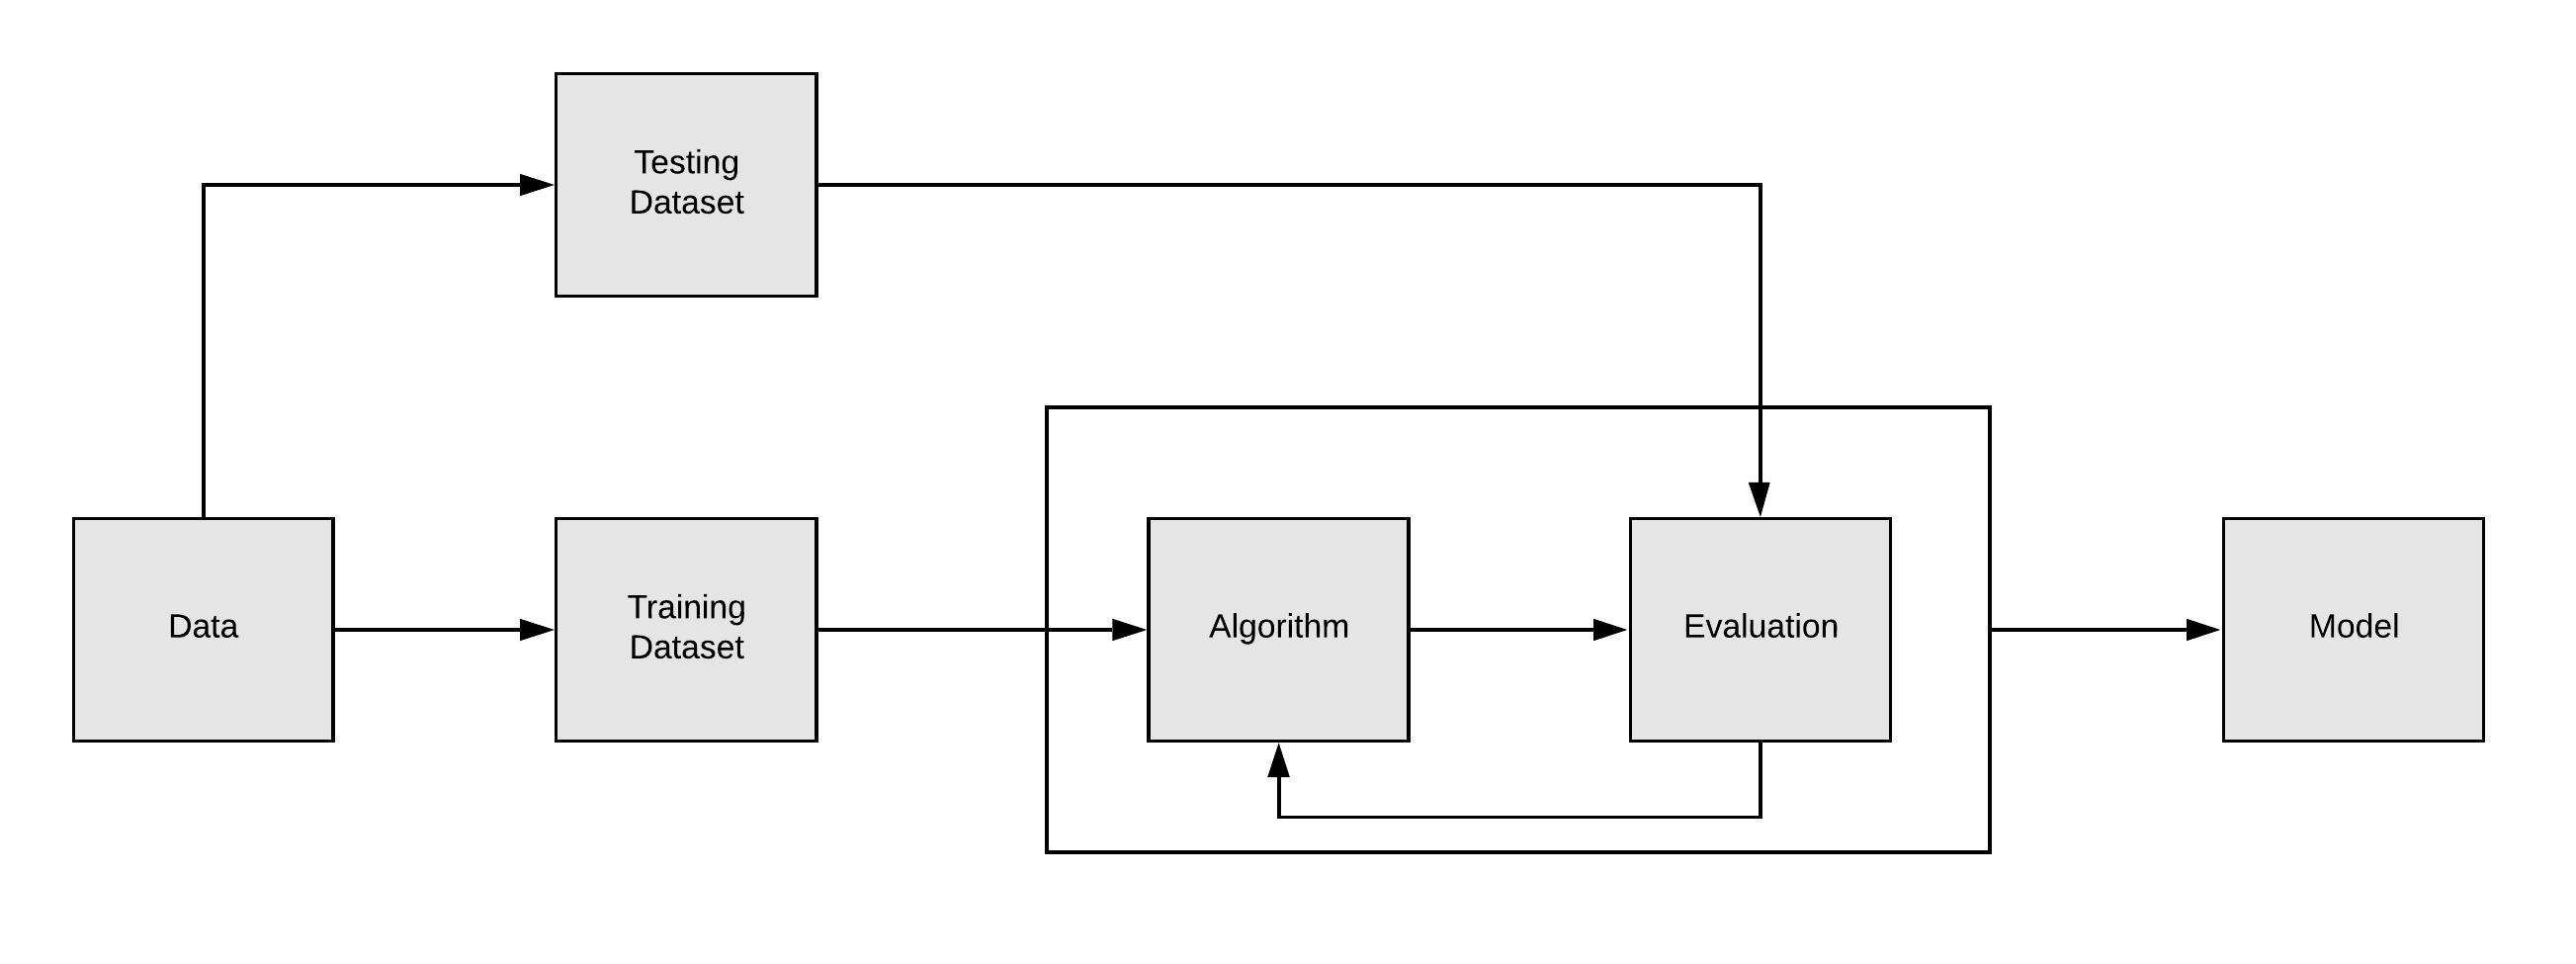
\includegraphics[width=16cm]{images/ML Workflow.jpeg}
    \caption{AutoML Workflow Diagram}
    \label{automl-workflow-diagram}
\end{figure}

Once, the data has been pre-processed, the dataset is split into a smaller subsets of the training dataset. One such subset is randomly chosen on which multiple algorithms are run to train and create a model for comparison and evaluation. Once the training and model creation of all chosen algorithms are completed, these models are evaluated based on multiple parameters one of which is their performance of an unseen data. When the performance metrics are calculated these models are evaluated and compared between each other and the best performing model is chosen for further training. Depending on the internal evaluation strategy of the AutoML tool used, more than one algorithm can be chosen for further training. Once these model(s) are chosen they are trained on various configurations of hyper-parameters using one of these search strategies; Grid Search, Randomized Search, Bayesian Optimization, etc. Once these models are trained and there hyper-parameters are optimised on the complete training dataset, they are evaluated against the testing dataset and the final best performing model is returned to the user.

%% a multi-line comment as an if statement
\if false

\section{Project Overview}
To tackle this repetitive and time consuming nature of these task, Dr. Joeran Beel proposed, what he called Federated Meta-Learning. Applying the concept of Federated Meta Learning, I have build an application called FMLearn to implement the same. Before explaining what the application is and what is does, some important information of this application are as follows. FMLearn is an application developed using the client-server model, which allows the exchange of meta-data about machine learning models and data for the purpose of meta-learned algorithm selection and configuration. In this Client-Server architecture the Client here is a popular Machine Learning package called Scikit-Learn which has been modified to the needs of the project. The client also enlists the help of another popular AutoML package for meta-data collection called Auto-Sklearn. 

\subsection{The Client: Scikit-Learn}
The client performs 2 crucial roles, one is to publish / send data to the server, which is then used by FMLearn to learn from and use this knowledge to make future predictions for tasks. The other task is to retrieve data from FMLearn, the data consists of Algorithm Predictions for previously seen or unseen datasets. The ideal choice for a client in such a role would be any popular and easy to use Machine Learning Library, and my choice was to use Scikit-Learn.

Scikit-learn \citep{scikit-learn} is a widely used, free and open source machine learning library\footnote{https://pypi.org/project/scikit-learn/}. I have used this as the client in the client-server model of my project to collect the information regarding how different classification, regression and clustering algorithms perform on various datasets and then publish / send this information about the model and other meta-data collected to the server - FMLearn - via the API endpoints which are made publicly available. It  also performs the role of retrieving the predicted algorithm for a previously seen or unseen task from the server via other exposed API's.

\subsection{The Server: FMLearn}
The server is a Python Application, which serves API's requests providing the caller with the requested details. It also acts as a knowledge base for all the data that is collected using the client, and learns from this knowledge base and suggests algorithms for a given task. It also has a very minimal user interface which explains the applications and provides links to various other useful information which might be required for the user.

\subsection{Meta-Features from Auto-Sklearn}
The tasks or datasets on which these algorithms run on are described by their meta-features which are obtained using the Auto-sklearn \citep{feurer:m} library via the client and this information about the meta-data about the data along with performance details of the algorithm on a particular task is sent / published to the server via an API call.

\fi

\section{Meta-Features}
\label{meta-feat-realted-work}
In the notion of Meta-Learning (MtL), Meta-Features are measures used to describe datasets and their relationship with algorithm bias. Meta-Features are used in Meta-Learning and AutoML tasks to describe the underlying dataset to create a machine learning, recommender systems and other models. The Meta-Features can be categorised to various groups, namely: General, Statistical, Information-theoretic, Model-based, landmarking, Relative Landmarking, Clustering, Complexity, etc. \citep{meta-features-1} \citep{meta-features-2} \citep{meta-features-3}. The most frequently adopted meta-features in three of the important categories used in this research are:
\begin{itemize}
    \item \textbf{General Meta-features}:
    Number of observations, Number of attributes, Number of output values, Dataset dimensionality.
    
    \item \textbf{Statistical Meta-features}:
    Standard deviation, Coefficient of variation, Covariance, Linear correlation coefficient, Skewness, Kurtosis
    
    \item \textbf{Information-Theoretic Meta-features}:
    Normalized class entropy, Normalized attribute entropy, Joint entropy of class and attribute, Mutual information of class and attribute, Equivalent number of attributes, Noise-signal ratio.
\end{itemize}

The Meta-Features discussed above are just a small sample of various possible characterisation features \citep{meta-features-1} \citep{meta-features-2} \citep{meta-features-3} , this is not an exhaustive list and details about these features are out of scope of this research.

\section{Related Work}

\subsection{Federated Meta-Learning}
Chen in \citep{chen-et-al} has used the term \textbf{Federated Meta-Learning} once before, but in a completetly different context. But the terms, Distributed Machine Learning \citep{disml} and Federated Machine Learning \citep{fedml-google} are realted to Federated Meta-Learning, in the sense that they share a few underlying concepts but yet totally different.

\subsection*{Distributed (Machine) Learning}
Automatic Learning has become popular and important in the recent years due to exponential growth of data being collected and the need to analyse data to create machine learning models. Peteiro in his survey of methods for Distributed Machine Learning \citep{disml}, points out that these needs introduced a new type of challenge with respect to efficiency and scalability of machine learning algorithms related to computational and memory resources. To solve this challenge researchers proposed two approaches, one is the concept of distributed machine learning algorithm which posses various limitations and the other strategy is to combine the outputs of various algorithms in a fashion similar to ensembling. On doing so large datasets can be addressed using a distributed clustering environment where both the techniques are used in combination to attain best possible results.

\subsection*{Federated Learning}
Federated Machine Learning \citep{fedml-google} is a collaborative learning strategy where a machine learning algorithm is trained across multiple devices which hold the data without exchanging it, i.e, the users remain the owners of the data. This approach is different to traditional approach of having a centralised repositories of data similar to OpenML \citep{OpenML2013} and also the approach of distributed machine learning where the it is assumed that the data is identically distributed across devices. Federated Learning allows the end users to build a common, robust model across devices without sharing data thus addressing important issues regarding data security and privacy.

\subsection*{Federated Learning vs Federated Meta-Learning}

Federated Machine Learning enables devices to collaboratively learn a shared prediction model while keeping all the training data on device, decoupling the ability to do machine learning from the need to store the data in a centralised server. Whereas Federated Meta-Learning provides an ecosystem where the learning happens locally on the users machine based on the dataset's meta-data that the user provides. This meta-data is used to make a recommendation of an algorithm that is used to create a model. Here, both the learning and data is kept on the users machine.


\subsection{Other Related Concepts and Research}
\subsection*{Algorithm Selection}

The field of algorithm selection and configuration is an area of intense research, according to Wikipedia, as stated by Rice in \citep{rice197665}, the process of algorithm selection is defined as:

\par\noindent\rule{\textwidth}{0.4pt}\newline
\textbf{Definition 1:} Given a portfolio ${\displaystyle{\mathcal{P}}}$ of algorithms ${\displaystyle{\mathcal{A}} \in {\mathcal{P}}}$, a set of instances ${\displaystyle{i \in {\mathcal{I}}}}$ and a cost metric ${\displaystyle{m:{\mathcal{P}} \times {\mathcal{I}} \to \mathcal{R}}}$, the algorithm selection problem consists of finding a mapping ${\displaystyle s:{\mathcal {I}}\to {\mathcal {P}}}$ from instances ${\displaystyle {\mathcal {I}}}$ to algorithms ${\displaystyle {\mathcal {P}}}$ such that the cost ${\displaystyle \sum _{i\in {\mathcal {I}}}m(s(i),i)}$ across all instances is optimized.
\par\noindent\rule{\textwidth}{0.4pt}

Rice, went into great detail about explaining about what he thought were the four major criteria in the selection process. The four primary criteria are as follows: Best Selection, Best Selection for a Subclass of Problems, Best Selection from a Subclass of Mappings and Best Selection from a Subclass of Mappings and Problems. He also proposed five major steps for analysis and solution of the algorithm selection process. These steps being: Formulation, Existence, Uniqueness, Characterization and Computation. He also explained in great detail about these criteria and steps using various example problem and formulating the best algorithm selection process for these criteria along with models. By doing this Rice in \citep{rice197665} proposed 15 questions that he suggested to be asked before an algorithm is chosen.

In \citep{kerschke2018automated}, Kerschke and others talks about algorithm selection problem by giving importance to \textit{per-instance algorithm selection problem} that is; given a computational problem, a set of algorithms for it, and a specific instance that needs to be solved, the problem is to determine which algorithm(s) can be expected to perform best on that instance. The authors also relates this type of problem to per-set algorithm selection, algorithm configuration, algorithm schedules and parallel algorithm portfolios and discusses about them in detail. By doing so in \citep{kerschke2018automated}, the authors also compare the results, discuss the problems faced and propose solutions for algorithm selection in discrete and continuous problems. They also provide an informative overview of problem specific feature set about which they discuss and provide a strong basis of why these characteristics are used in algorithm selection. They also shed some light on various other applications and there contributions based on there impact in this ever growing and evolving field of algorithm selection.

The propositional satisfiability problem or SAT is an NP-Complete problem, and in \citep{xu-et-al} the authors propose an automated approach for constructing per-instance algorithm portfolios for SAT and proposed a online platform called SATzilla. Here the authors propose a new approach to algorithm selection based on the idea of building an approximate run-time predictor compared to the previous "winner-takes-all" approach. In the winner-takes-all approach where the algorithms run-time is measured on a representative set of the problem and which ever algorithm performs better takes the top spot. The approximate run-time predictor is an heuristic approximation to the perfect solution and the authors built an empirical hardness model, which is a computationally inexpensive predictor of an algorithm’s run-time and it based on features of the instance and past performance of the algorithm.

ASLib \citep{bischl-et-al} is a benchmark library for algorithm selection, which focuses on (not a limitation to) constraint satisfaction problems. The authors introduced 12 algorithm selection scenarios from six different areas and discussed the format and showed examples for automated exploratory data analysis that will run for each new scenario that has been submitted to there ASLib platform. Their platform also facilitates algorithm selection methods by providing a common set of benchmarks and tools. The authors built on top of Rice's \citep{rice197665} formalisation of algorithm selection and also took a different approach then that of SATzilla \citep{xu-et-al}. SATzilla approach was to select a single algorithm for solving the problem instance, ASLib, tries to find a schedule where ordering and time budget where all or a subset of the all the algorithms can be executed in a to reflect the expected performance of the given algorithm.

\subsection*{AutoML}

Though the above mentioned researchers laid the foundation for algorithm selection, these researches either discussed about the problem in general or focused on one particular field like the propositional satisfiability or SAT problem(s). Due to the growing demand in commercial use of Machine Learning, various enterprises have aimed to satisfy the AutoML problem, this has lead to the increase in research and development of tools which help novices to use machine learning without the expertise required.

According to \citep{feurer:m} and \citep{kotthoff:l}, new methods for increasing efficiency and robustness of AutoML are the current trend and focus in this area of research. The authors proposed tools like Auto-Sklearn and Auto-WEKA respectively to solve the problem of algorithm selection by improving on the existing AutoML methods. In Auto-Sklearn \citep{feurer:m}, the authors made improvements to the AutoML approach by introducing Meta-learning, which they used to find good instantiations of machine learning algorithms, which is a complementary approach to that of Bayesian optimization techniques. In another approach the authors of Auto-Sklearn used automated ensemble construction, where they used the models created during the evaluation process, instead of discarding these models they used the models in a post-processing technique to create an ensemble which is evaluated during optimization and from there results they found that the ensemble almost always outperformed individual models. 

In Auto-WEKA \citep{kotthoff:l}, the authors built on the Bayesian Optimisation approach. They used the Tree-structure Parzen Estimator (TPE) approach which a Sequential Model-Based Optimization (SMBO) algorithm, they also used Sequential model-based algorithm configuration (SMAC) models, which were used to create probabilistic models. These two types of models gave robust performance for algorithm selection and probabilistic estimators for hyper-parameters respectively, which were used to demonstrate the feasibility of an automatic approach to learning algorithm and hyper-parameter selection. The result of this research was a tool called Auto-WEKA, which has a list of 47 WEKA classification algorithms that were used as a single learning algorithm, which selects a single base classifier and a meta- or ensemble- classifiers. It was one of the first tools to perform a fully automated algorithm selection and hyper-parameter optimization for a large set of candidates.

\subsection*{Meta-Features}

Rivolli in \citep{meta-features-3} surveys a comprehensive list of meta-features and how they are used in classification problems, they authors also analyse and organise the meta-features by highlighting there positive and negative attributes of each meta-feature. They also defined what a meta-feature is, and it is as follows:

\par\noindent\rule{\textwidth}{0.4pt}\newline
\textbf{Definition 2:} Let ${\displaystyle{D \in \mathcal{D} }}$ be a Dataset, ${\displaystyle{m: \mathcal{D} \to \mathcal{R}^{k'}}}$ be a characterisation measure, and $\displaystyle{\sigma: \mathcal{R}^{k'} \to \mathcal{R}^{k}}$ be a summarisation function. Both $\displaystyle{m}$ and $\sigma$ have also hyper-parameters associated, $h_m$ and $h_\sigma$ respectively. Thus, a meta-feature $\displaystyle{f: \mathcal{D} \to \mathcal{R}^{k}}$ for a given dataset $\displaystyle{\mathcal{D}}$ is given by:

\begin{center}
    $\displaystyle{f(\mathcal{D}) = \sigma(m(\mathcal{D}, h_m), h_\sigma)}$
\end{center}
\newpage
The measure $\displaystyle{m}$ can extract more than one value from each data set, i.e., $\displaystyle{k'}$ can vary according to $\displaystyle{\mathcal{D}}$, which can be mapped to a vector of fixed length $\displaystyle{k}$ using a summarisation function $\displaystyle{\sigma}$.

\par\noindent\rule{\textwidth}{0.4pt}

The authors also present a tool called Meta-Feature Extractor, which can be used to measure the meta-features proposed and discussed in this paper and made the tool publicly available to the users as a package in Python and R.

The authors in \citep{meta-features-1} and \citep{meta-features-2} introduce concepts about meta-features characterisation and selection algorithm respectively. Castiello in \citep{meta-features-1} analyses most commonly used meta-features and discusses there properties an inherent manner. He also introduces new features by transforming the existing features as a result of their analysis. The author(s) also suggest a set of measures that can be used to describe a dataset using the proposed meta-features. The suggested meta-features can be used as a bias for other base-learning in for their respective tasks. 

Filchenkov in \citep{meta-features-2} creates an optimal meta-feature suggestion algorithm for different cases. The authors do this by creating a new approach for meta-feature engineering, which they also have proved to be useful for feature selection algorithm's recommendation. They also conduct an almost complete analysis of most of the popular meta-features and use the results so obtained to suggest optimal meta-features for different tasks. One of the major contributions by this paper is the analysis they have done in relation to classification algorithms. They have used various popular classification algorithms for which the author(s) engineered new meta-features and recommended existing meta-features for most of the popular algorithms and they categorised this specific type of measures as model-based meta-features.

%% a multi-line comment as an if statement
\if false

\section{Related Research}

\subsection{Paper1}
\subsection{Paper2}
\subsection{Paper3}
\subsection{Technology1}
\subsection{Technology2}

\section{Technology Used}
\subsection{why this stack}
\subsection{why client-server model}
\subsection{why scikit learn}

\fi



\chapter{Design and Implementation}

This chapter provides details regarding the FMLearn application, implementation of the proposed concept, that is, Federated meta Learning and it's working mechanisms. Each component of the application is discussed in detail including the components that were considered and tested, but are not a part of the final experimentation. Explanation of all the design decisions are provided in detail so as it make it easier for the reader to understand how the application developed over-time and reached it's final state. The FMLearn application attempts to solve the issue of redundant work put in by developers to find the best algorithm and it's hyper-parameters, repeatedly for a previously solved / optimised dataset, and possibly suggests algorithms for a previously unseen dataset as well. If this is achieved, the users of this application and the community in general will be greatly benefited by saving time spent waiting for program to complete, saving electricity consumed on the running the machines and cooling them, the computational power expended over a repetitive task and money spent in all of the above is saved in finding the best algorithm and it's hyper-parameter.

The design and implementation choices led to the development of a working prototype of the concept Federated Meta-Learning and the application FMLearn. The server was developed in python and is used to portray the capabilities of the application. The concept of Federated Meta-Learning discussed in \ref{federated-meta-learning} and the changes in the workflow of a typical Machine Learning project caused due to the introduction of Federated Meta-Learning is discussed in section \ref{fml-workflow}. Then we discuss in detail the prototype FMLearn which was built to demonstrate this concept under section \ref{fmlearn}, while discussing it's architecture design in section \ref{architecture} along with some design decisions in section \ref{design-decisioins} and why these were taken. We will also be discussing in detail about the Model built by FMLearn to predict / recommend the potentially best algorithm(s) for a given task along with it's workflow. In section \ref{scikit-learn} we will be discussing in detail about the modifications made to scikit-learn so that it can act as a client to FMLearn along with discussing the data description used.

\section{Federated Meta-Learning}
\label{federated-meta-learning}

Federated Meta-Learning focuses on learning algorithm performance measures for arbitrary tasks. Essentially federated meta learning is an ecosystem where the raw data is kept on the original devices and the meta data and performance metrics of the algorithm on the tasks would be stored on a central FML server. Using this historic performance data, predict the best performing algorithm along with its hyper-parameters for a previously seen or unseen task.

The input to Federated Meta-Learning is a description of the task, and the output is a recommendation for the potentially best performing algorithm(s) to solve that task. This recommendation could consist simply of a list of the best algorithms, or their predicted performance values. The list could also consist of multiple sub-lists created with different meta-learners.

In its simplest form, federated meta-learning would simply be a knowledge base or directory of algorithm-dataset performance measures. Ultimately, Federated Meta-Learning would be able to predict algorithm performance for unseen tasks.

\section{Workflow of Federated Meta-Learning}
\label{fml-workflow}

From section \ref{workflow-automl}, we know that a typical algorithm selection and configuration task using the AutoML tools result in a repetitive and time consuming process which in turn eats up a lot of computing resources, electricity and money. To tackle this problem the concept of Federated Meta-Learning as seen in section \ref{federated-meta-learning} can be applied. When we take this concept and apply it to the current ecosystem of Machine Learning tasks we get a workflow as show in Figure \ref{fml-workflow-diagram}.

\begin{figure}[t]
    \centering
    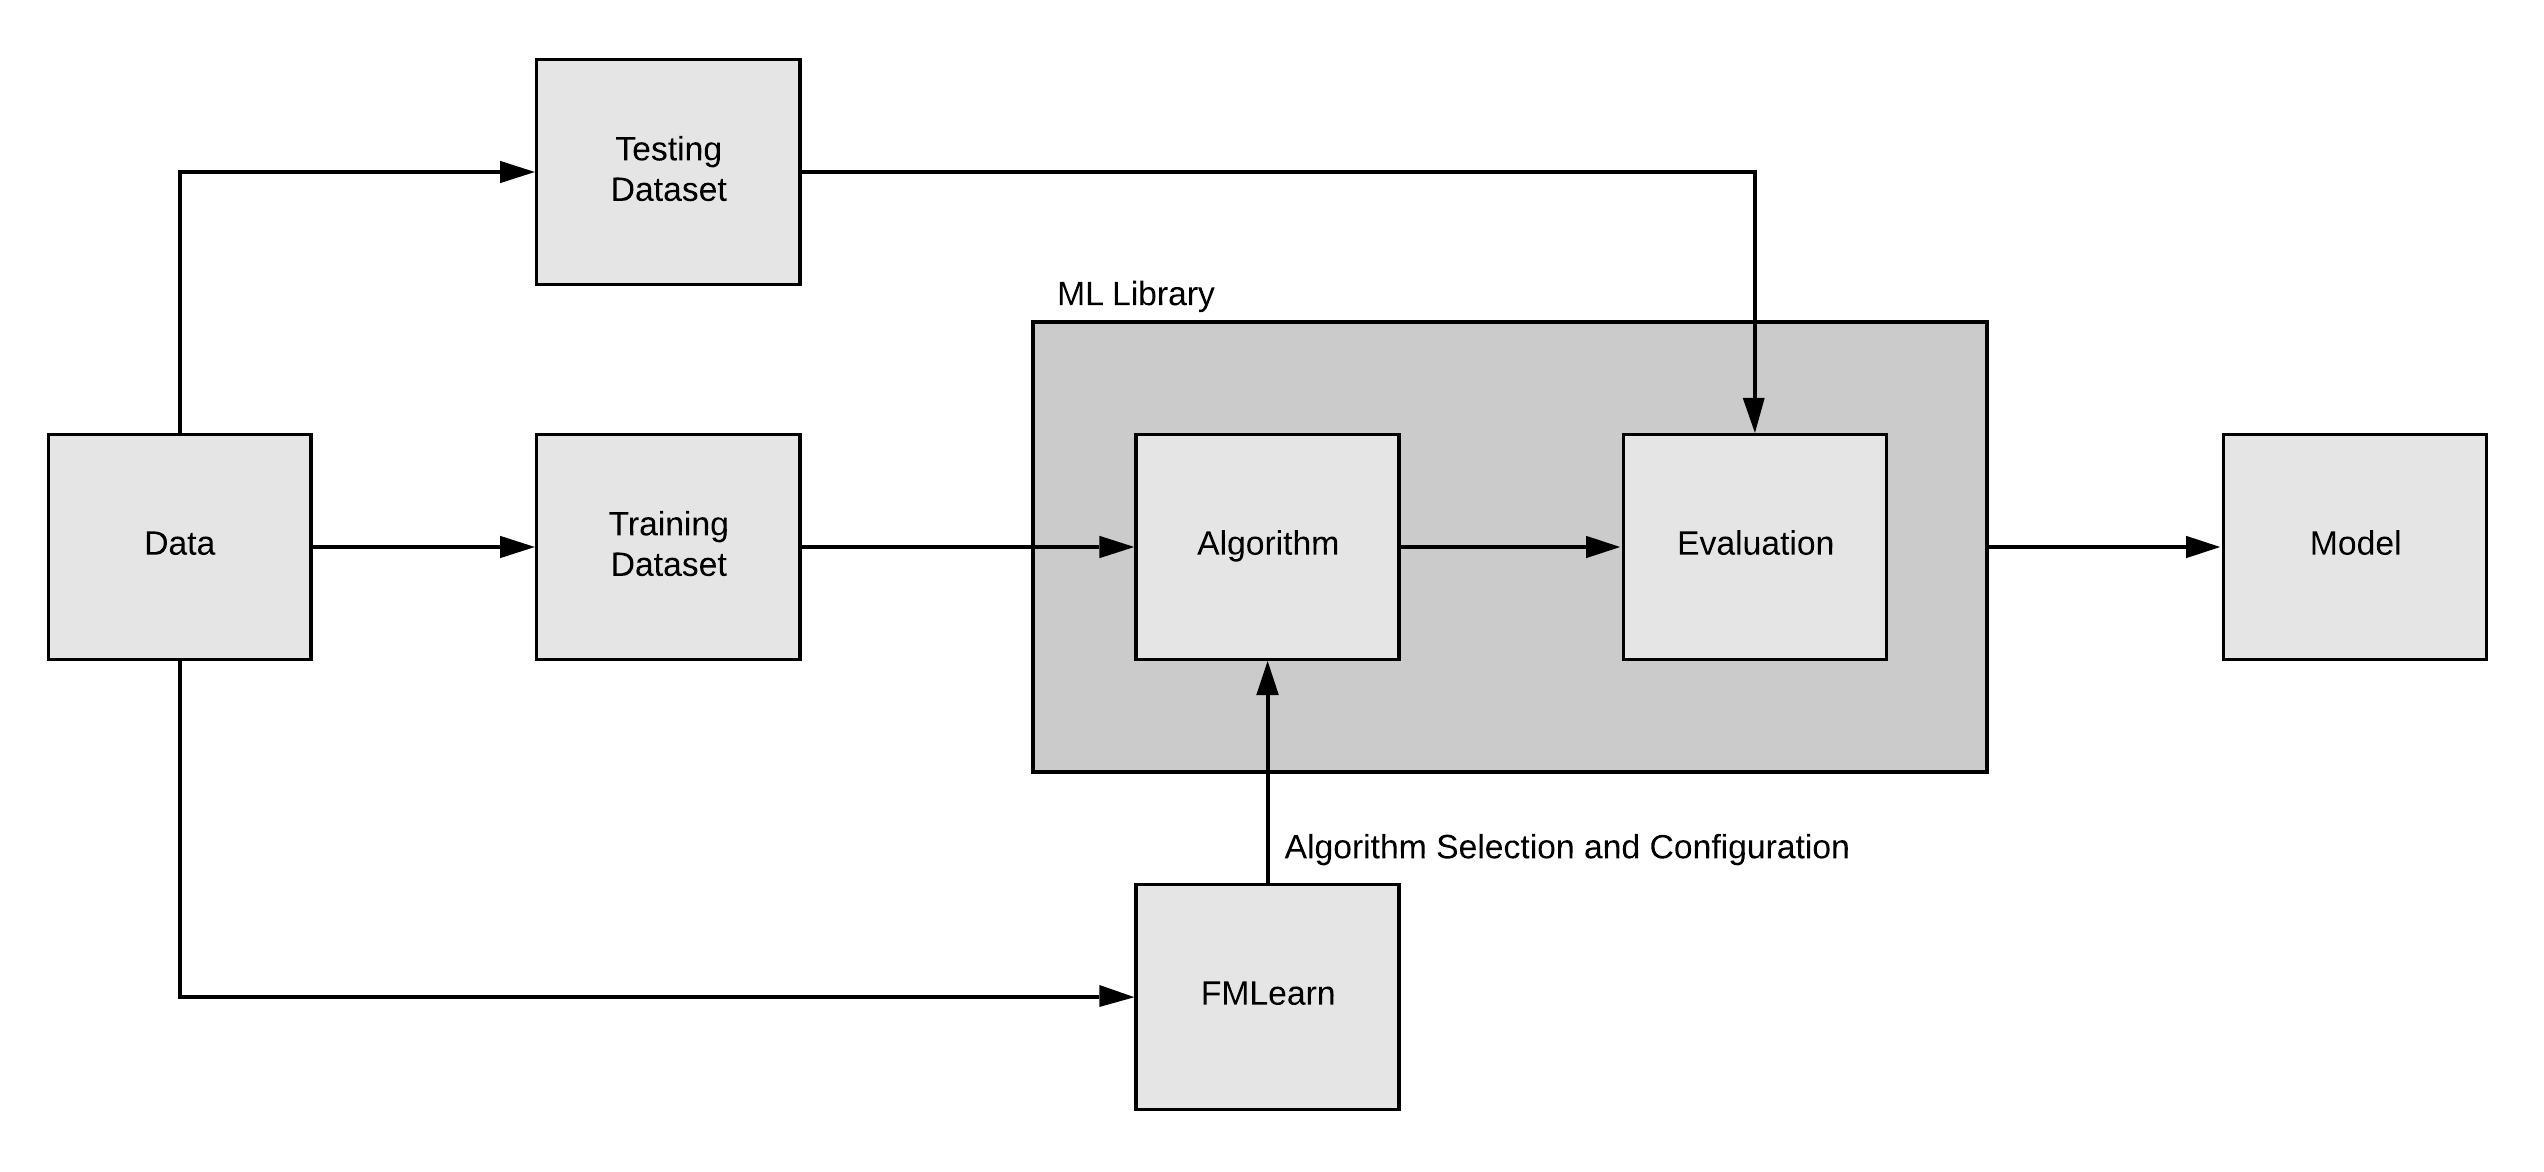
\includegraphics[width=15cm]{images/FML Workflow.jpeg}
    \caption{Federated Meta-Learning Workflow Diagram}
    \label{fml-workflow-diagram}
\end{figure}

Let's go into detail about the workflow of Federated Meta-Learning, Initial steps of the workflow remain similar to the working of AutoML (as seen in section \ref{workflow-automl}). The data is split into training and testing datasets, the training dataset in first sent to the library for the purpose of model creation. Here, the dataset is pre-processed using various techniques like data-cleaning, data imputation, data encoding, feature selection, feature exploration, feature engineering, feature co-relation, etc.

The difference between the 2 processes arise at the point when the data is obtained. The data apart from being sent to the library for pre-processing it is also sent to the Federated Meta-Learning application after finding the meta-features of the dataset. Once these meta-features are obtained Federated Meta-Learning predicts / recommends the potentially best performing algorithm(s) along with it's hyper-parameters for the given dataset. Once this recommendation is received by the Machine Learning library it re-optimises the algorithms and builds the model based on the training dataset which was received after pre-processing and this model is then evaluated against the testing dataset and then the final model is returned to the user.

The major difference with the workflows described in Figure \ref{automl-workflow-diagram} (as seen in the Section \ref{workflow-automl} - Workflow of AutoML Libraries) and Figure \ref{fml-workflow-diagram} is the introduction of an external application which applies the concept of Federated Meta-Learning. This application results in the elimination of the repetitive nature of algorithm selection and configuration task, which would drastically reduce the time spent on such a task along with the computational resources, electricity and money spent here.

\section{FMLearn}
\label{fmlearn}

FMLearn is an application which is a simple proof of concept of Federated Meta-Learning. FMLearn allows everyone to benefit from the data that is generated through machine learning and data science libraries. FMLearn is built using the Distributed Application Architecture (DAA), following the Client-Server Model. This allows the users to access as well as to exchange information and services with others. Though a Peer-To-Peer Model would be possible, this design was avoided due to the limitation in time as well as favouring the ease of development using the client-server model.

FMLearn consists of a client which in our case a modified version of the popular Machine Learning library Scikit-Learn, but it could be any machine learning library. The Server is a Python Flask Application which handles all API calls and Data Store requests made by the user. FMLearn also acts as a knowledge base, storing all the algorithms-data performance measure collected though the machine learning library. The server also provides publicly available API's which can be accessed by any Machine Learning or Data Science tool to use FMLearn irrespective of the programming language used to build them to get a recommendation for the potentially best performing algorithm(s) and it’s hyper-parameters to solve it’s task without being constrained by the need to use the client that is supported by this paper (modified scikit-learn).

\subsection{Design Decisions}
\label{design-decisioins}

A few important Design Decisions that needs to be addressed before proceeding with further discussions are as follows:

\begin{itemize}
    \item Why Client-Server Model?
    
    The biggest design decision was taken in the early stages of the dissertation. A decision was taken to proceed with the Client-Server model rather than a Peer-To-Peer model with respect to the architecture design of the application. This was an "Experience Based Design" as I have prior experience working with Client-Server Application model and more importantly due to the limited availability of time and ease of development which cannot be achieved when a Peer-To-Peer architecture is followed.

    \item Why Scikit-Learn?
    
    Scikit-learn is a free software machine learning library for the Python programming language \citep{scikit-learn}. It is also among the popular and easy to use python libraries available in the market. Though other libraries with similar capabilities are available in the internet scikit-learn was chosen as an "Intuition Based Design" due to familiarity with the library and it's easy to use nature.
    
    \item Why a Public API Server?
    
    The concept of Federated Meta-Learning \citep{fml}, was envisioned as an ecosystem where everyone would benefit from the data that is generated though Machine Learning libraries and the prediction of the best performing algorithm along with it's hyper-parameters be available to all. A public API server ensures that even if the developers aren't using the supported client - modified scikit-learn - they can still benefit from the recommendations made by FMLearn.
    
    \item Why not a stand-alone client?
    
    A stand alone client was a possible aim for this dissertation, as said the client doesn't highly depend on the features provided by scikit-learn, though a few dependencies exists. But this idea was dropped due to limited availability of time to concentrate on building and improving the server where the recommendations were to be made.
    
    \item Why Flask?
    
    Flask is a popular, extensible web micro-framework for building web applications with Python \citep{flask} and is among the most used web applications frameworks in python. It was a choice between Django and Flask, and Flask was chosen because of ease of use in terms of quick development when compared to Django. This was a "Reference Based Design" decision and when trying out both frameworks it was easier to get things started with Flask as opposed to Django. It is also easy to deploy Flask on to a free hosting services like Heroku, for the application to go live.
    
    \item Why PostgreSQL?
    
    PostgreSQL is a free and open-source relational database management system. It is easy to use when compared to other options and most importantly as it is a widely used database it was also available as a database deployment option in various online hosting platforms such as Heroku.
    
\end{itemize}

These are among the major design decisions made in the early stages of the dissertation which needed to be addressed before proceeding. Though a few other design decisions were made during the process of development they will be explained as and when the appropriate section of the application is discussed.

\subsection{Architecture Design}
\label{architecture}

The figure \ref{architecture-diagram} describes the client-server architecture of the FMLearn application as a whole, along with a few other components that haven't been discussed yet, these components will be introduced here and will be expanded upon later sections of this report. 

From the Figure \ref{architecture-diagram} we can see that the entire application is divided into two major chunks the client and the server. The client here is the modified version of Scikit-Learn which is explained in Section \ref{scikit-learn} in detail. To which I have introduced an additional package called `\texttt{fmlearn}`. This package provides the user with the capability to interact with the server. This package also functions as an important link to the intermediary step where the data description is obtained for a given dataset or task i.e., the dataset is converted into it's meta-features. The conversion of dataset to it's Meta-Features is handled by a 3rd party library called Auto-Sklearn \citep{feurer:m}. Auto-Sklearn is an external library, a dependency is introduced here, details about it will be further explained in Section \ref{auto-sklearn}.

\begin{figure}[t]
    \centering
    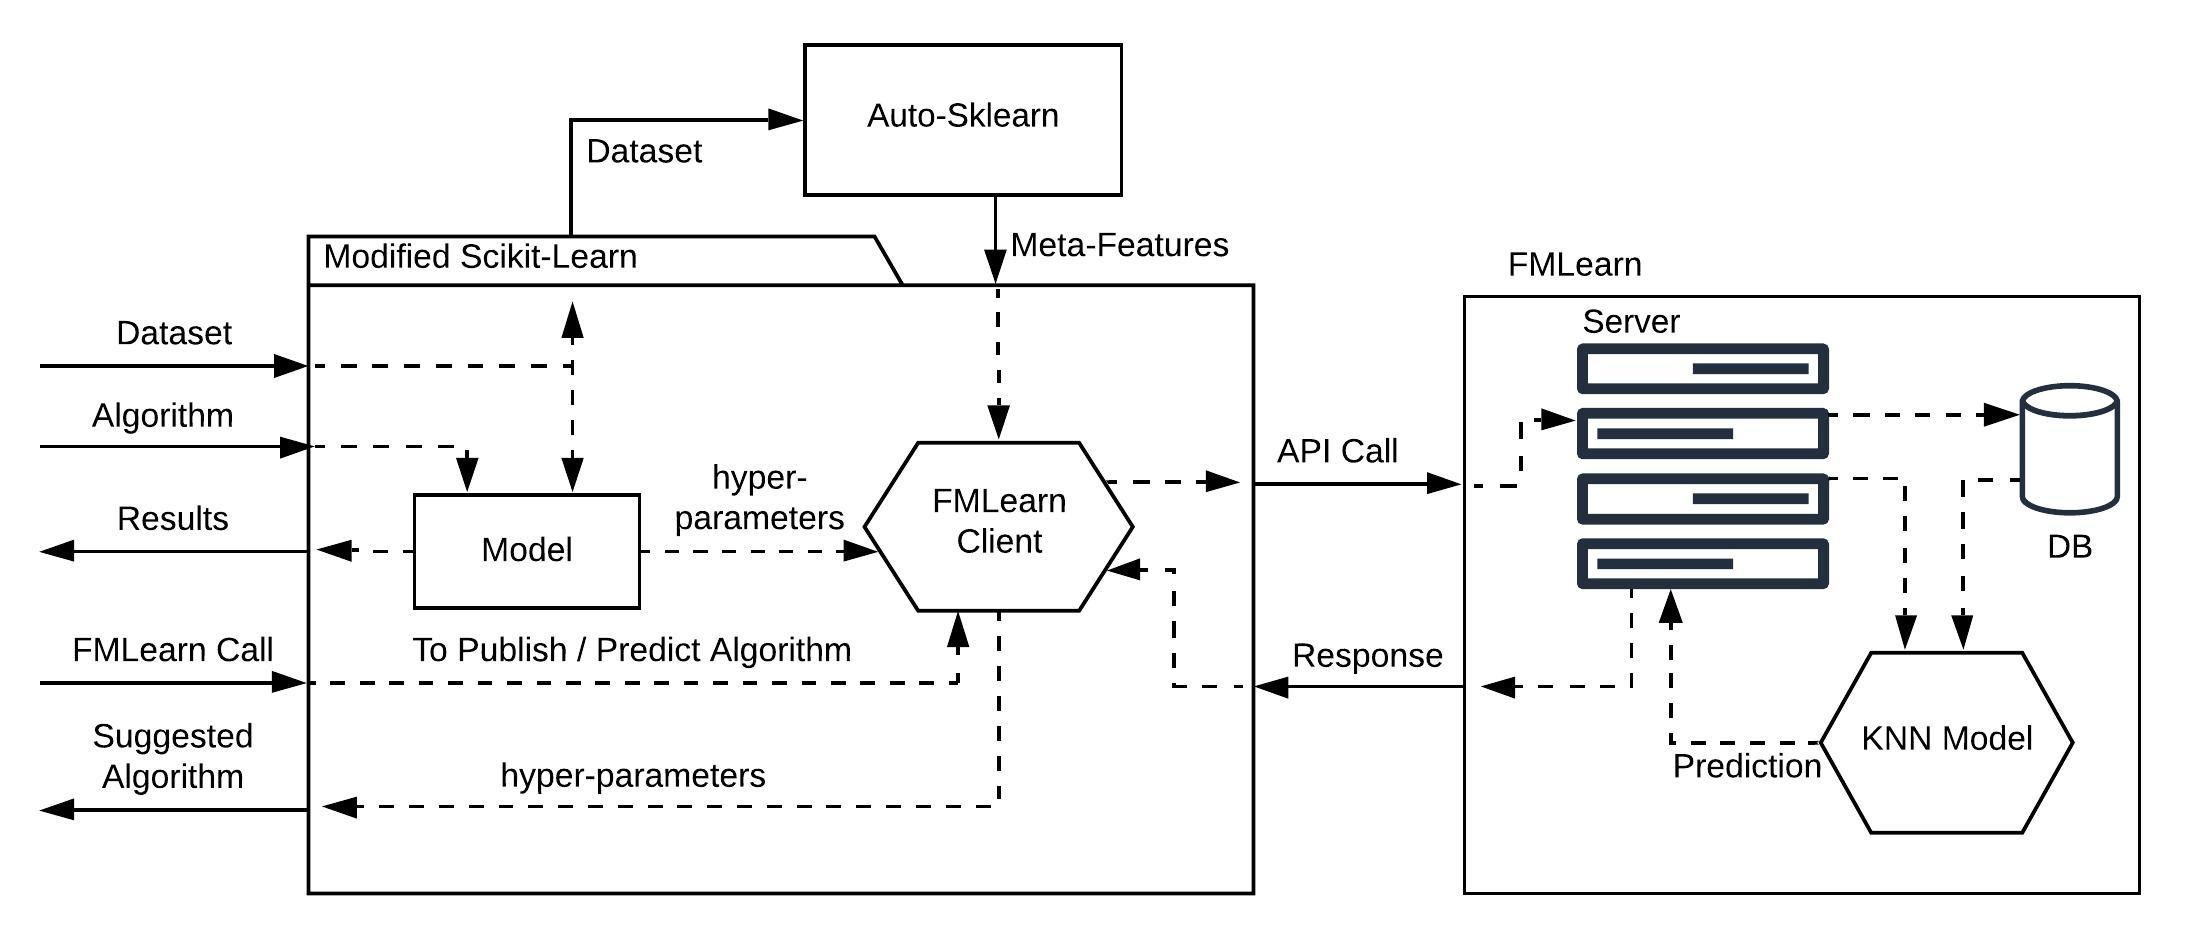
\includegraphics[width=15cm]{images/FML Architecture Diagram.jpeg}
    \caption{Architecture Diagram}
    \label{architecture-diagram}
\end{figure}

\subsection*{FMLearn Client}

The client majorly performs 2 tasks, publishing the data to the server and displaying the results obtained for algorithm recommendation from the server to the user. Irrespective of the task, the \texttt{fmlearn} module obtains the dataset from the user and it is converted to it's Meta-Features with the help of Auto-Sklearn. Depending on the task the user might want a recommendation of the best performing algorithm or might want to contribute his findings to the betterment of the FMLearn in general. Depending on the use case either an API call is made to obtain the recommendation for the user or the model details along with the performance metrics which is obtained from the user and the model directly, then an API call is made to publish these details to the server respectively.

\subsection*{FMLearn Server}

The server performs various roles depending on the task and is explained in Section \ref{fmlearn-server} in detail. The server primarily acts a recommender system, recommending algorithm(s) for a given task. The server also acts a knowledge base or directory of algorithm-dataset performance measures, apart from this is also provides API's to expand or build this knowledge base. This knowledge base is stored in a PostgreSQL Database and is also used to build a Machine Learning model. The model was built using the K-Nearest Neighbors algorithm. The details about the model and algorithm in general will be discussed in the Section \ref{knn-model}. This model is used to make recommendations to the users for previously seen or unseen task or dataset. The model's ability to recommend the best performing algorithm(s) have been exposed to the public via API's.


\section{The Client: modified Scikit-Learn}
\label{scikit-learn}

In this Client-Server Architecture, the stable release of the client i.e., modified version of scikit-learn is available on GitHub via the following link:
\begin{center}
\href{https://github.com/mukeshmk/scikit-learn/releases/latest}
{\texttt{https://github.com/mukeshmk/scikit-learn/releases/latest}}.
\end{center}

The complete code repository is available at: \href{https://github.com/mukeshmk/scikit-learn/}{\texttt{https://github.com/mukeshmk/scikit-learn/}} \newline which is forked from: \href{https://github.com/scikit-learn/scikit-learn}{\texttt{https://github.com/scikit-learn/scikit-learn}}.

After downloading the stable release and installing the library by following the instructions specified in the \texttt{README.md} file, we can use it normally as we use scikit-learn, since it's a fork of the original release it has all the features of the stable release plus it has the features of FMLearn.

\subsection*{Initialisation of FMLearn}

To initialise \texttt{fmlearn}'s client we have to import the \texttt{FMLClient} package from \texttt{sklearn.fmlearn} and then create an object of the class \texttt{FMLClient} as follows:
\begin{lstlisting}
    # imports the FMLearn client into the program
    from sklearn.fmlearn import FMLClient
    # initialises the client
    fmlearn = FMLClient()
\end{lstlisting}

\subsection*{Obtaining the Meta-Features}

Once the client as been initialised irrespective of the task the first thing to do would be do tell \texttt{FMLearn} what dataset we will be using for the task this can be done as follows:

\begin{lstlisting}
    # assuming that the import for train_test_split has been done
    # and the data has been loaded and split into 'X' and 'y'
    x_train, x_test, y_train, y_test = train_test_split(X, y, test_size=0.2, random_state=12)

    # this is a function introduced by the Client to let FMLearn know 
    # what dataset is being used for the task.
    fmlearn.set_dataset(x_train, y_train, x_test, y_test)
\end{lstlisting}

Setting the dataset using the \texttt{sets\_dataset()} method triggers a background call to an external 3rd party library called Auto-Sklearn which is used to describe the Dataset and obtain the Meta-Features for that dataset. This is further explained in Section \ref{auto-sklearn}. These Meta-Features thus collected is then sent to the server to be processed as required.

\subsection*{Available Methods}

Depending on the objective of the user, the user can proceed with his program in one of these two ways:
\begin{enumerate}
    \item Get recommendation for a task.
    \item Publish performance data for a task.
\end{enumerate}

\subsection*{Recommendation for a Task}

If the user wants to get a recommendation for a task all they would have to do is to call the method \texttt{predict\_metric()} as follows:

\begin{lstlisting}
    # this method returns the recommendation of the
    # best performing algorithm along with its hyper-parameters
    # for the dataset set using the set_dataset() method
    fmlearn.predict_metric()
\end{lstlisting}

This method provided by the client internally makes an API call to the server, sending the server the Meta-Features of the dataset which was obtained from \texttt{auto-sklearn}. Upon reaching the server, the server processes the request, responding with the appropriate algorithm recommendation which is then sent to the user as shown in Figure \ref{sample-output}. The recommendation can then be used by the user to create a model with the specified algorithm and the hyper-parameter values. The created model can then be used by user to proceed with the task after re-optimising the parameters to suite the users dataset.

\begin{figure}[H]
    \centering
    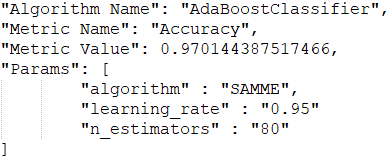
\includegraphics[width=9cm]{images/sample-output.png}
    \caption{Sample Output}
    \label{sample-output}
\end{figure}

\subsection*{Publish Metrics for a Task}

If the user wants to publish a performance metric for a task which they performed, the user can do so by using the \texttt{publish()} method by passing the model used, scoring metric and the score as it's parameters as follows:

\begin{lstlisting}
    # the `model` parameter contains the model trained using the dataset
    # `fmlearn.ACCURACY` specifies the evaluation metric used
    # the `score` parameter contains the evaluation results.
    fmlearn.publish(model, fmlearn.ACCURACY, score)
\end{lstlisting}

Upon calling the client's \texttt{publish} method the meta-features of the dataset, model details including the algorithm name, hyper-parameters, along with the evaluation metric and the evaluation scores are sent to the FMLearn server. This data is processed and stored in the database, which is later be used to build a model.

\subsection{Data Description: Auto-Sklearn}
\label{auto-sklearn}

As discussed in section \ref{meta-feat-realted-work}, Meta-Features describe the dataset, and there are various dedicated tools which provide the required features. One such tool is Auto-Sklearn \citep{feurer:m}. It is an open-source AutoML tool written in Python that automatically determines effective machine learning pipelines for classification and regression datasets. Though this is an AutoML tool, it was used here for it's \textbf{meta-learning} step in the AutoML pipeline, which it uses to warm start the Bayesian optimization procedure in it's core. This meta-learning step. i.e., obtaining meta-features is abstracted inside all the features provided by the tool and is not easily available to the users to use outside the tool.

Meta-features provided by Auto-Sklearn fit the following meta-features categories: General, Statistical and Information-Theoretic meta-features, though a few meta-features exists outside these categories, but majority of them fall into these. An utility package was introduced inside the FMLearn's client (modified Scikit-Learn) to make use of the functionality provided by auto-sklearn to obtain the meta-feature of a dataset. This utility function performs the input checks, transforms the data and performs the required validations before passing on the dataframe to Auto-Sklearn's calculate meta-features method. It is available in this package via the imported method.
\newline
\begin{lstlisting}
            from autosklearn.metalearning.metafeatures.metafeatures 
            import calculate_all_metafeatures_with_labels
\end{lstlisting}


The input to the \texttt{calculate\_all\_metafeatures\_with\_labels()} method is the dataset and the output is a set of meta-features. These meta-features are then converted into the required format and then forwarded to server via API calls. A few of the meta-features thus obtained are: \texttt{ClassEntropy, ClassProbabilityMean, NumberOfMissingValues, NumberOfCategoricalFeatures, NumberOfNumericFeatures, etc}. Depending on the dataset there can be about 24-30 meta-features obtained for a given dataset. Refer appendix \ref{meta-features-ask}, for the complete list of meta-features and to see a an example of values obtained via the Auto-Sklearn.

The end user is abstracted away from existence of this feature, the call to auto-sklearn is handled internally by the client upon letting the client know about the dataset in use.

\begin{lstlisting}
    # this is a method provided by the FMLearn client that internally calls
    # `calculate_all_metafeatures_with_labels()` method provided by auto-sklearn
    # which provides the meta-features required.
    fmlearn.set_dataset(x_train, y_train, x_test, y_test)
\end{lstlisting}

\subsection*{Design Decision}

Before finalising with \texttt{auto-sklearn} another library by Hadi called \texttt{dataset2vec} \citep{dataset2vec} was explored and evaluated for it's effectiveness in model building. This library represents a tabular dataset in a hierarchical fashion by defining a dataset as a set of features, where each feature is a set of instance values. Working with this library proved to be quite challenging due to the lack of documentation and lack of pre-trained model which converts the dataset to it's meta-features and thus making it necessary for the user to train a model. Though this paper claimed to out-perform the current state-of-the-art, a design decision was made to not use \texttt{dataset2vec} and instead proceed with \texttt{auto-sklearn}, as a model was available and also a support by the community to improve the meta-feature extraction model.

\section{The Server: FMLearn}
\label{fmlearn-server}

The stable release of the server - FMLearn in this Client-Server Architecture is available on GitHub via the following link:

\begin{center}
\href{https://github.com/mukeshmk/fm-learn/releases/latest}
{\texttt{https://github.com/mukeshmk/fm-learn/releases/latest}}.
\end{center}

The complete code repository is availabe at: \href{https://github.com/mukeshmk/fm-learn}{https://github.com/mukeshmk/fm-learn}. The application is also deployed on Heroku. Heroku is a platform as a service (PaaS) that enables FMLearn to available on the cloud to be accessed by everyone. The application is deployed and available via the link mentioned below, though this is an API server a basic user-interface has been developed so as to provide information about Federated Meta-Learning and API documentation.

\begin{center}
\href{https://fmlearn.herokuapp.com/}
{\texttt{https://fmlearn.herokuapp.com/}}.
\end{center}

\subsection*{API's Provided}

The server provides several API's among which two of the important API's are the \texttt{publish} and \texttt{predict} API's. These API's represent the two important functionalities of the proposed prototype. 

\subsection*{Publish API}

The \texttt{publish} API solves the problem with the workflow of machine learning and data science libraries. These libraries usually work in isolation and the information regarding how an algorithm performs on a particular dataset is neither publisher nor shared. 

\begin{lstlisting}
# the input JSON object to publish API
{
	"algorithm_name": algorithm_name,
	"dataset_hash": dataset_hash,
	"meta_features": [
		{
			"feat_name": feature_name,
			"feat_value": feature_value
		}
	],
	"metric_name": metric_name,
	"metric_value": metric_value,
	"params": [
		{
			"param_name": hyper_parameter_name,
			"param_value": hyper_parameter_value
		}
	],
	"target_type": target_type
}
# NOTE: "meta_features and params" are a list of objects
# but for illustration purpose only 1 item has been shown.
\end{lstlisting}

The publish API can be called from within these libraries as done in the modified scikit-learn presented and thus enabling the users to share the algorithm performance data. The API is a \texttt{POST} method which can be accessed via this endpoint \texttt{/metric} and takes a JSON object as input in the format as described above.

\subsection*{The Underlying Database}

The input data is validated, preprocessed and stored in the database. A PostgreSQL database used in this application which contains 3 tables to store the information received from the client. These tables are structured as follows as shown in Figure \ref{class-diagram}. The three tables are \texttt{Metric}, \texttt{Meta Feature} and \texttt{Params}, the \texttt{Metric} table has a one to many relation ship with both the \texttt{Meta Feature} and \texttt{Params} tables and this relationship puts the database in it's 3rd Normal Form.

\begin{figure}[H]
    \centering
    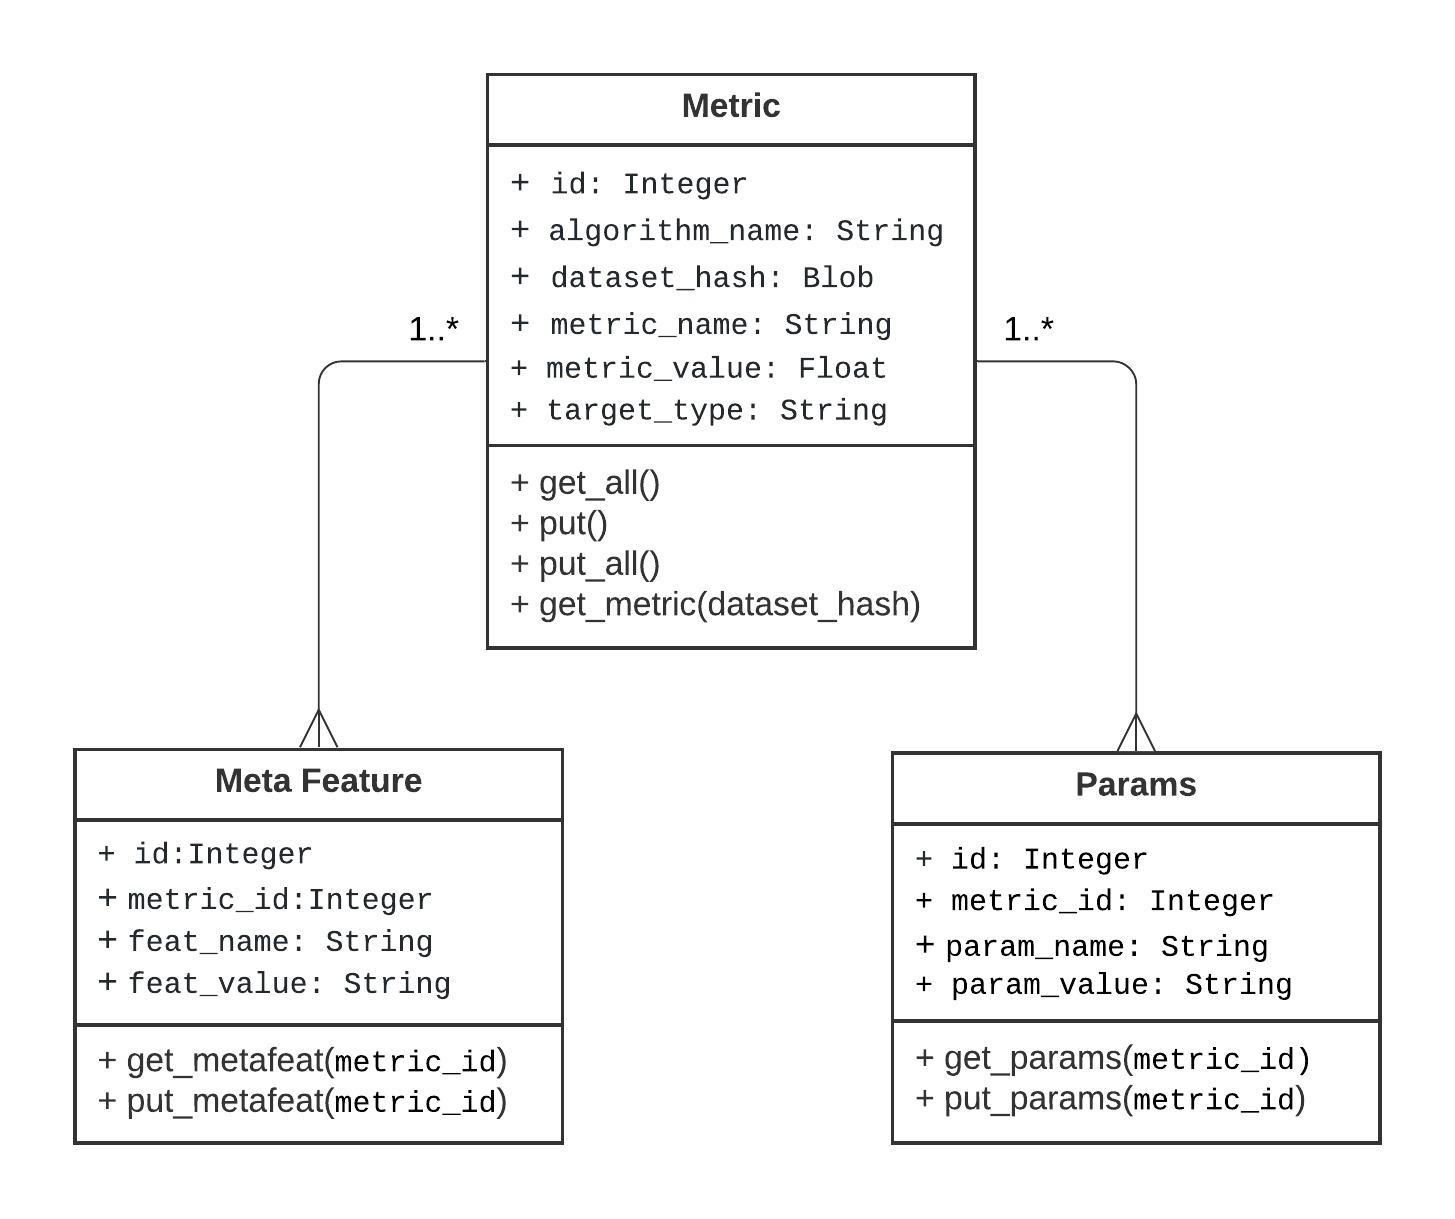
\includegraphics[width=15cm]{images/Class Diagram.jpeg}
    \caption{Class Diagram}
    \label{class-diagram}
\end{figure}

This database thus created acts as a knowledge base which contains information about the algorithm-data performance metrics. FMLearn also provides others API's to access this data which enables sharing of performance details of various algorithms among software libraries. The response of this API when there are no internal errors is a JSON object similar to the request object with a HTTP status code of 200.

\subsection*{Predict API}

The \texttt{predict} API solves the problem with the repetitive nature of the workflow of machine learning libraries, where the algorithm selection and hyper-parameter optimization tasks are to be performed repeatedly. The \texttt{predict} API can be called by the machine learning libraries, as done in the modified scikit-learn presented in this paper, and thus breaking the cycle and saving time, electricity, computation power and money. The API is a \texttt{GET} method which can be accessed via this endpoint \texttt{/metric/predict} and the API accepts a JSON object as input which is similar to the below format:

\begin{lstlisting}
# the input JSON object to predict API
{
	"dataset_hash": dataset_hash,
	"meta_features": [
		{
			"feat_name": feature_name,
			"feat_value": feature_value
		}
	],
	"target_type": target_type
}
# NOTE: the key "meta_features" accepts a list of objects
# but for illustration purpose only 1 item has been shown.
\end{lstlisting}

This input is validated, preprocessed and then sent to the model for the best algorithm prediction (this is discussed in detail in Section \ref{knn-model}) and the result of the prediction is sent to the user as the best algorithm recommendation for the given task. This response is a JSON object in the following format:

\begin{lstlisting}
# the output JSON object of predict API
{
  "recommendations": [
    {
      "algorithm_name": algorithm_name,
      "metric_name": metric_name,
      "metric_value": metric_value,
      "params": [
        {
          "param_name": hyper_parameter_name,
          "param_value": hyper_parameter_value
        }
      ],
      "target_type": target_type
    }
  ]
}
# NOTE: "recommendations and params" are a list of objects
# but for illustration purpose only 1 item has been shown.
\end{lstlisting}

\subsection{KNN Algorithm}
\label{knn-model}

The goal is to use FMLearn to try and find the closest existing dataset which is very similar to the dataset for which an algorithm is to be recommended. Then recommending best performing algorithm for the requested dataset is based on the closest existing dataset. FMLearn doesn't try to predict the best performing algorithm rather tries to predict the closest dataset, this is an important point to be noted in the algorithm recommendation process. Prediction of an algorithm along with their hyper-parameters using a machine learning model might not be feasible as there are various types of machine learning problems like classification, regression and clustering just to name a few. These problem types employ various algorithms within each type, which have varying performances and the resulting model will be a multi-class output problem. This problem will be to try and predict algorithm name, metric used, metric value, and not to mention the parameters of an algorithm. This will result in a lot of mismatch with the hyper-parameter suggestion and the output recommended will just be a random set of values. This might become feasible given the existence of a huge dataset and a complicated neural network, but gathering this data is out of scope of this dissertation. Here, in this dissertation we are building the first proof of concept for Federated Meta-Learning. Thus predicting the closest existing dataset for the input dataset and then finding the best algorithm for that dataset is the best possible approach in the given scenario.

The algorithm used to make prediction or recommendation of the best performing algorithm for a given task is the \textbf{K-Nearest Neighbours (KNN)} algorithm. KNN is a supervised, non parametric learning algorithm, meaning, the target variable is known and that it does not make an assumption about the underlying data distribution pattern. In the case of FMLearn, a KNN classification algorithm has been used with k=1 and the distance between points is calculated using Euclidean distance. The "K" in KNN is the number of nearest neighbors to which the given input point must be the closest to before labeling the input point. In terms of FMLearn, "K" represents the number of datasets that the input dataset has to be closest to. Since we want to find one dataset to which the input dataset is closest to we are setting the value of "k=1". 

\subsection*{Design Decision}
To guarantee reliable recommendations of algorithms based on historic performances of algorithms-data pairs, K-Nearest Neighbours algorithm and a Support Vector Machine were ideal choices to being with. Both KNN and SVM were tested with FMLearn. Though in it's current state FMLearn has a very small dataset with a low dimensionality or small number of features, both algorithms perform equally well. A decision was made to go with KNN over SVM because on the long run, when the number of instances or points in the dataset increase KNN begins to outperform in a low-dimensional space, whereas as SVM might face difficulty is finding a linear separation in the dataset when the number of points increase. Though KNN is very sensitive to bad features and outliers, in this case we know that all the features being used to build the model are required to describe the dataset and are obtained from auto-sklearn and as for the case of outliers, since K value being used in KNN is one, outliers will not be a major factor and will not affect predictions or algorithm recommendations. Whereas, in the case of SVM, which is generally considered to be a better performer than KNN, the drawbacks arise when the number of points increase, even if a smart kernel is used, the number of output classes that get created increases as the number of new datasets or variations of datasets seen by FMLearn increase. This puts SVM in a huge disadvantage as the need arises to create separating planes for each class. Thus for these reasons KNN was chosen over SVM as the algorithm of choice for recommending the best performing algorithm for the user.

\subsection*{Algorithm Recommendations}

Recommending the best algorithm falls into 3 different possibilities based on the closes of the input dataset, which can be categorised as follows:
\begin{itemize}
    \item Previously known dataset.
    \item Previously unknown dataset, which is similar to a known dataset.
    \item Previously unknown dataset, which is dissimilar to a known dataset.
\end{itemize}

In the case of a previously known dataset for which the best algorithm is also known, the distance between the points is 0 units, thus making the predictions 100\% accurate. Whereas, for previously unknown dataset which is highly similar to known dataset the prediction of algorithm is accurate but the hyper-parameters require re-optimisation to suite the new dataset. But, in the case of an unknown dataset which is highly dissimilar to a known dataset, the model is able to predict the type machine learning problem the dataset belongs to, but not the best algorithm for it, instead it recommends a set of algorithms which it thinks are the best suited in this case instead of recommending a single algorithm.
   

\subsection{Pre-Processing and Model Building}
\label{model-building}

The data-frame which is the sent to the KNN Algorithm consists of the following features: meta-features and target type as input and the output is the dataset hash. The meta-features consists of a maximum of 29 features, if the feature doesn't exist of the dataset, the missing value is imputed with -1. The other pre-processing done are as follows the meta-feature values are scaled between 0 and 1, the feature "Target Type" is one hot encoded and the output variable "Dataset Hash" is label encoded. Since we are only trying to find the closest dataset the repeated datasets are removed based on the dataset hash, thus retaining the variations of the same dataset. The pre-processed dataset is sent to model for training and later used for prediction of the dataset. Based on the predicted dataset, FMLearn suggests the best performing algorithm to the user.

The model training and re-training is an automated process in FMLearn. The model is retained when a trigger from the database is sent to the application. This trigger is set off, after every 10 new records that are added to the database (this number is configurable though the \texttt{config file}). This enables FMLearn to keep improving it's model and it's predictions as and when new data is published to it, thus improving the recommendations.

\section{FMLearn Workflow}

The Figure \ref{sequence-diagram} represents the Sequence Diagram of the application, explaining the object interactions in a time sequences. The sequence diagram of FMLearn represents 2 major use cases. Each use case represents the flow of object interactions in the case of where the user wants to:
\begin{itemize}
    \item publish data to FMLearn
    \item get a recommendation from FMLearn for a given dataset.
\end{itemize}

Though the working of each individual modules/objects have been discussed in previous sections of this report, this section focuses explicitly on giving a in-depth understanding of how all the individual modules work together to form FMLearn.

\begin{figure}[t]
    \centering
    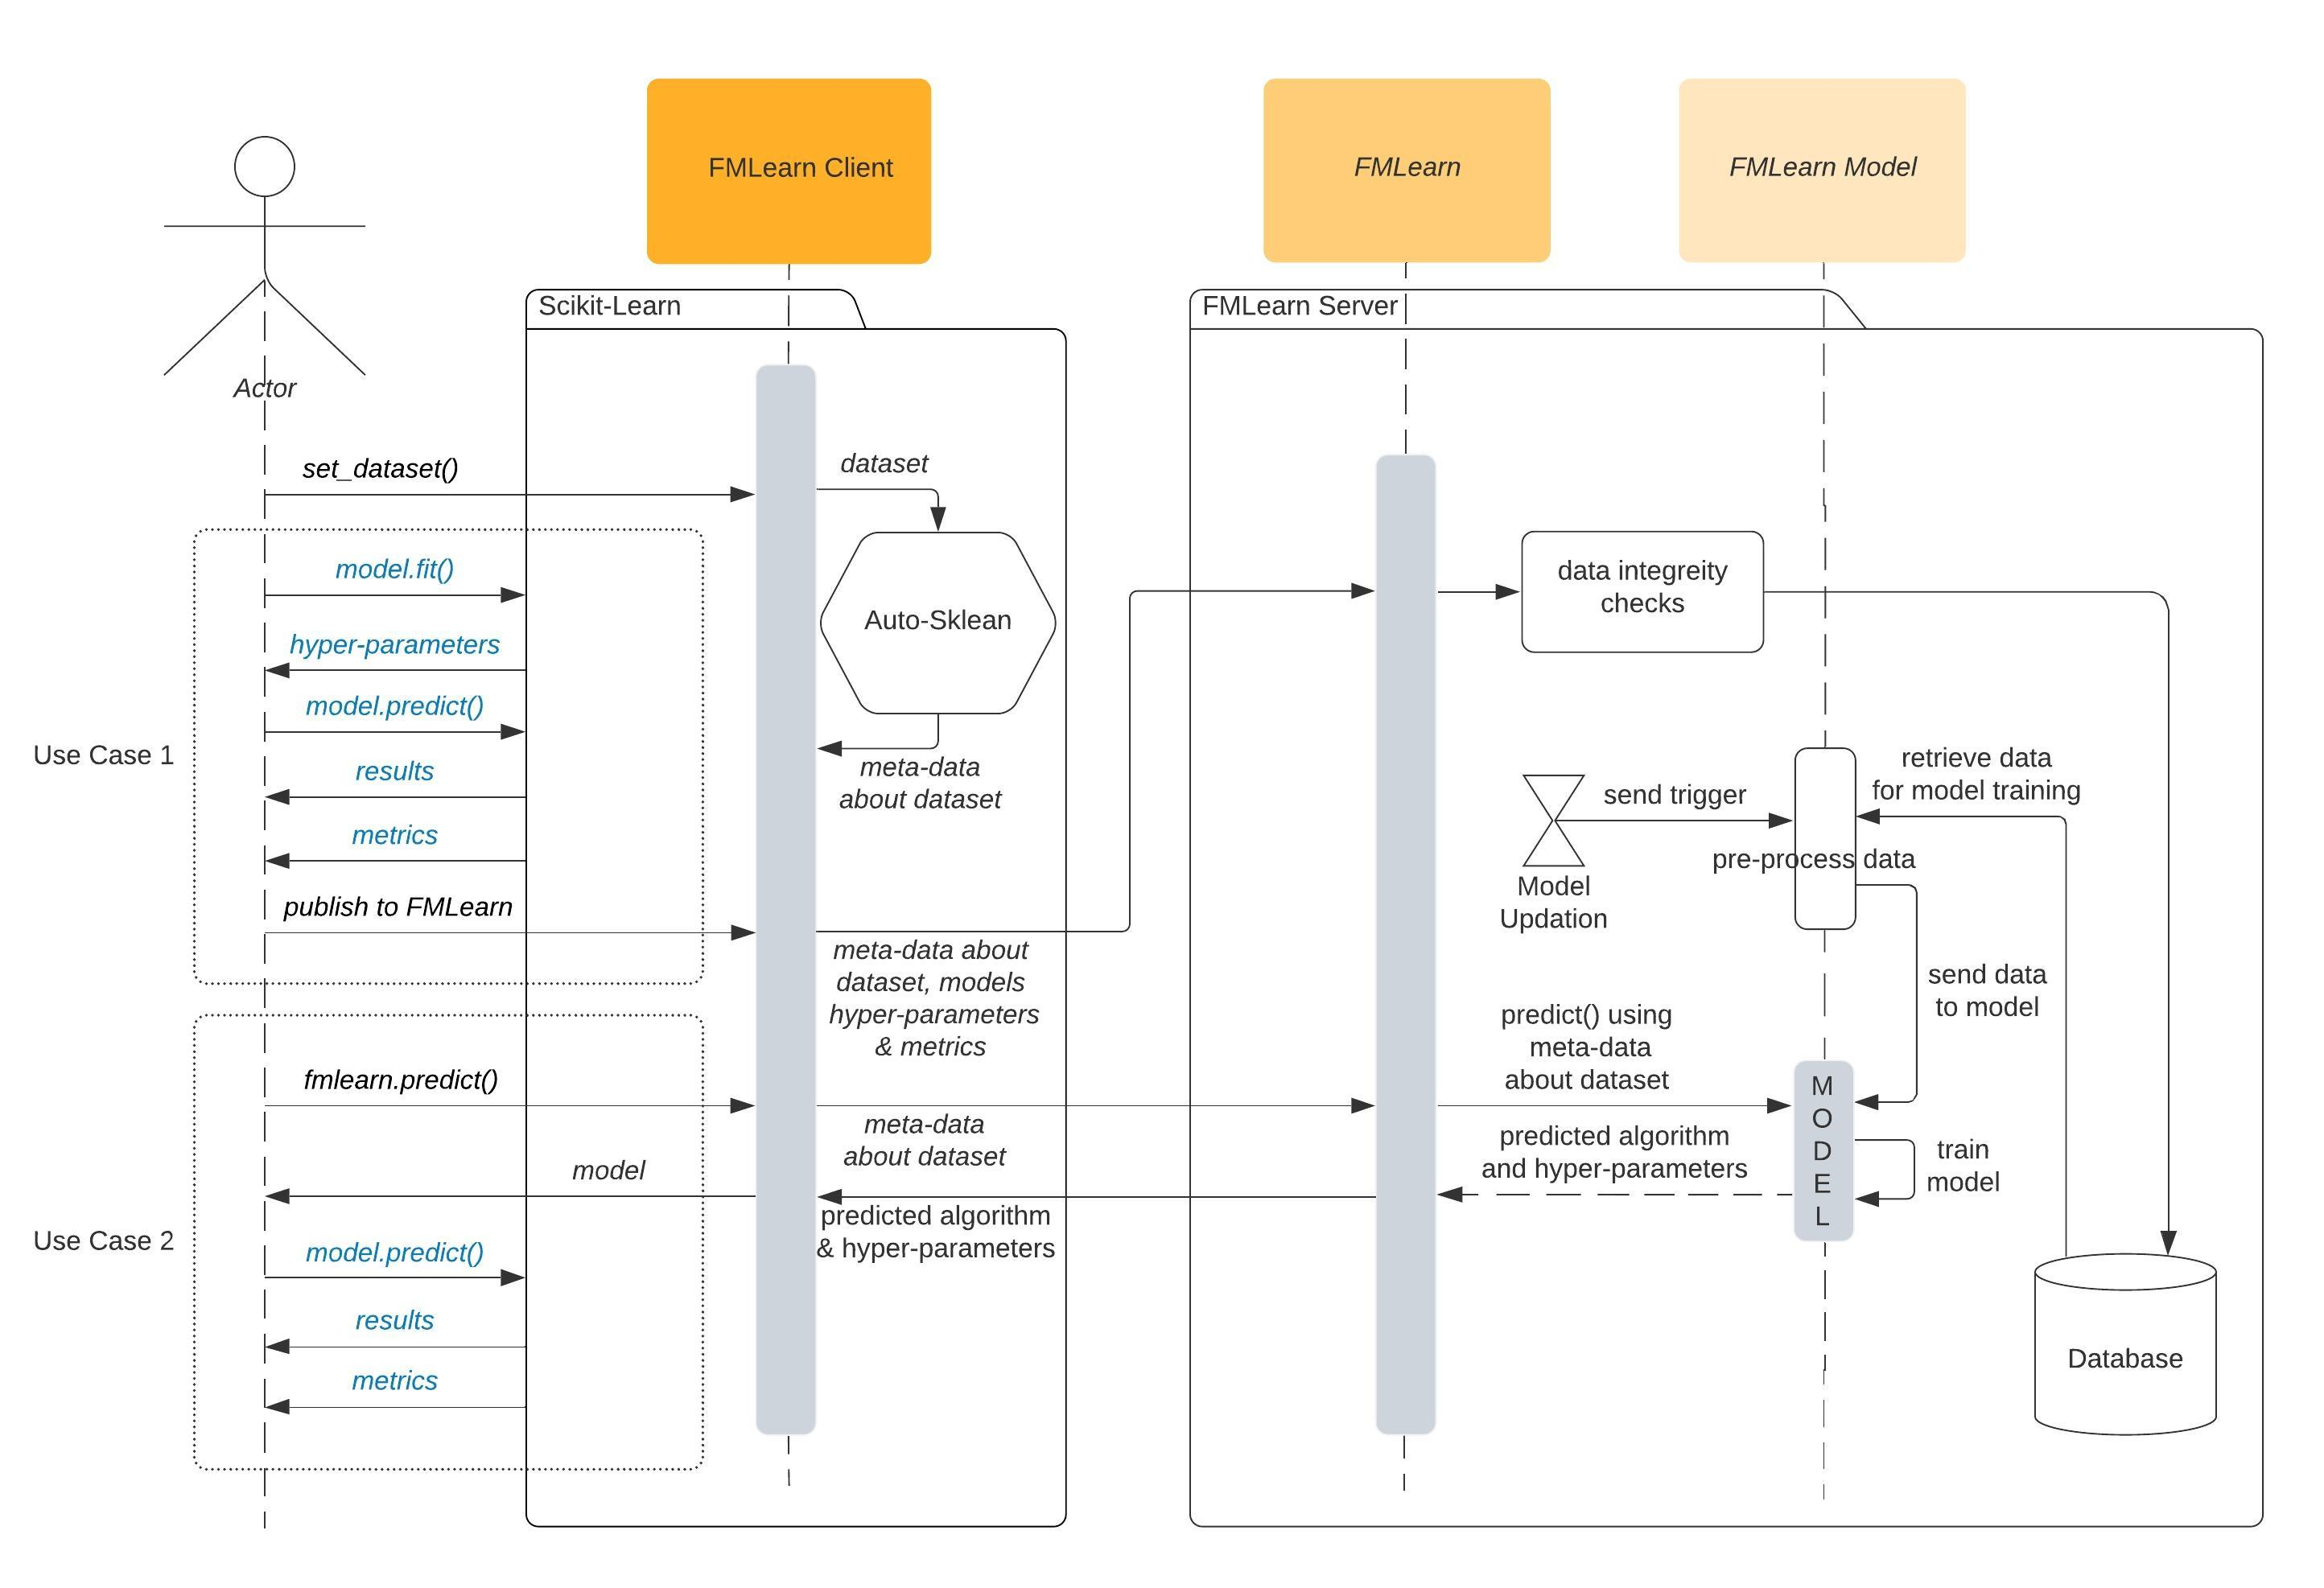
\includegraphics[width=15cm]{images/Sequence Diagram.jpeg}
    \caption{Sequence Diagram}
    \label{sequence-diagram}
\end{figure}

\subsection*{Use Case 1: Publish Metric}

The use case 1 describes the scenario where the user wishes to publish their algorithm-data metrics to the FMLearn application. The first step of this process is to let FMLearn know about the underlying dataset by using the method \texttt{set\_dataset()}. As explained in section \ref{auto-sklearn}, it makes an internal call to \texttt{Auto Sklearn} to find the meta-data / meta-features about the dataset. These meta-features are stored in the FMLearn client object created and are later used when publishing. Then the user performs his preprocessing tasks, finds the best algorithm along with it's hyper-parameters and uses the model so thus created to evaluate the results using the \texttt{model.fit()} and \texttt{model.predict()} methods for the created model objects the results. This model, along with it's results is sent to FMLearn's client via the \texttt{publish()} method, where model details like the algorithm used and hyper-parameters are extracted and a request object is created with them along with the meta-features obtained from auto-sklearn and the algorithm metrics. This request object is a JSON object which is used to make an API post call to the FMLearn server. Once the server receives the request object it's pre-processed and checked for the data integrity and then pushed into the database and a \texttt{200 OK} response is sent to the client.

\subsection*{Use Case 2: Predict Metric(s)}

The second use case characterises, the scenario where the user wishes to get a recommendation from the FMLearn application for the best performing algorithm for his dataset. The first step here as well is to let FMLearn know about the underlying dataset by using the method \texttt{set\_dataset()}, this obtains the meta-features of the dataset and stores them in the client object. The next step is to make a call to the client to get the recommendation using the \texttt{predict()} method. This creates a JSON request object which contains the meta-features which is sent across by the client to the FMLearn server via an API call as discussed in section \ref{fmlearn-server}. Upon being received by the server, the request object is pre-processed and checked for data integrity. The pre-processed data is sent to the model built using KNN algorithm (discussed in section \ref{knn-model}) to make predictions about the closest dataset available, upon finding the closest dataset, the best performing algorithm for the predicted dataset along with it's hyper-parameters are retrieved from the database and an response JSON object is created and sent to the client. The client then recommends the received algorithm to the user, which the user then further re-optimises if required and then proceed with his task.


\section{Security and Privacy Concerns}
FMLearn is a client-server architecture-based \citep{clientserver} application which provides public API’s for it's users, and it brings its own security and privacy concerns. The different aspects of security and privacy issues that are to be considered with respect to FMLearn are - but not limited to:

\begin{enumerate}
    \item A client-server architecture.
    \item Publicly available API server \citep{input-validation} (which could be broken down)
\end{enumerate}

\subsection{Security Concerns}

FMLearn was built using Python Flask, and uses PostgreSQL, which acts as the public API server which exposes various API to users to use the application and is currently hosted on Heroku .

One of the most important security concerns with the current implementation of FMLearn is that the users have unlimited access to APIs (Flash Crowd Problem) \citep{flash-crowd}, this could have severe consequences. A denial of service is possible, and extraction of all information of few of the major effects. This could be resolved using various rate-limiting strategies:

\begin{itemize} 
    \item Limiting per connection property (IP address)
    \item Limiting per user (account / access token / API key)
    \item Limiting per application property (user account / resource type)
    \item Limiting based on context (region / type of app)
\end{itemize}

Once these rate-limiting features have been introduced if someone tried to repeatedly access the API, they would get the following error.

\par\noindent\rule{\textwidth}{0.4pt}
\begin{center}
\texttt{HTTP/1.1 429 Too Many Requests}\\
\texttt{Retry-After: 3600}
\end{center}
\par\noindent\rule{\textwidth}{0.4pt}

Rate limiting prevents malicious code from abusing legitimate / illegitimate access to the API.

One of the basic and yet most powerful technique which helps to prevent a lot of security issues is Input validation \citep{web-application-sec}. Input validation should act as the first line of defense in case of a malicious attack. It is also useful to reject malicious data which helps prevent DoS attacks by rejecting unreasonably large inputs and against injection attacks by rejecting crafted payloads. Some of the possible Input validation techniques which could be easily enforced in my case are:

\begin{itemize}
    \item Enforcing sensible length limits on inputs.\\
    (i.e., 2MB of user’s hashed dataset is not allowed)
    \item Enforcing strict content types on provided data inputs.\\
    (i.e., an API expecting JSON data should not accept anything else.
    \item Enforcing strict data type checking on inputs.\\
    (i.e., Numbers should be numbers, and SQL code as input results in an error)
\end{itemize}

Even though input validation is a decent first line of defense, it will fail if used as the only line of defense because when the application evolves and brings in complex input types it will not prevent attacks as it will be complex to determine the validity of complex data at input time. Moreover, complex validation procedures usually suffer from bypass attacks, and making validations might break functionality. \citep{philippe_2020}

\subsection{Data Protection}
Another possible issues specific to FMLearn is the storage of hash for the complete dataset in the proposed prototype, the dataset is hashed using sha256 though this is very secure it has its own set of vulnerabilities \citep{sha256} that need to be taken into consideration, for now we can assume that sha256 is safe to use. But if it is broken there is a possibility that all the user data can become compromised. Even if the hash of the dataset is not broken, but if the meta-data about the model (like the model parameters) and dataset is available to the hacker, it is very much possible that a model could be reconstructed and the data of the user can be compromised.

Currently FMLearn is also vulnerable to Eavesdropping Attack, this is because the data sent from scikit-learn to FMLearn is not encrypted and is in plain-text, so various sniffing tools like Wireshark, Nmap, etc., can be used to monitor the network traffic and sniff the data transmitted between client and the server. To prevent such attacks, I can use a technique similar to twitter’s developer API access, where in the user is required to create an account with FMLearn and is required to use certain keys generated during account creation:

\par\noindent\rule{\textwidth}{0.4pt}
\begin{center}
\texttt{ACCESS\_TOKEN = ''\\}
\texttt{ACCESS\_TOKEN\_SECRET = ''\\}
\texttt{API\_KEY = ''\\}
\texttt{API\_SECRET\_KEY = ''}
\end{center}
\par\noindent\rule{\textwidth}{0.4pt}

This introduces a 3-legged oauth authentication workflow similar to twitter’s developer API \citep{twitter-oauth} access and these tokens can them be used to securely transfer data back and forth between the client and server, without worrying about eavesdropping attack. But then by introducing this we bring in new security vulnerabilities into the application which needs to be addressed separately in a larger scale. But for now sticking to just encrypting the information related to dataset let it be dataset hash or meta-data about the data, can be done as the first step in the necessary direction for this dissertation to proceed using public key encryption techniques. Doing just this helps protect the privacy of the user’s data from potential sniffers and maintains the integrity of the data over the network.

The scope of improvement in terms of security is huge in this project, it can be made secure enough for users to confidently use, but all this is just until things don’t go wrong.

\subsection{Social Concerns}
In the long run, social questions need consideration such as preventing manipulation of the data, developers of algorithms may have an interest that their algorithms are "recommended" to other users. So, the developers might manipulate data so the underlying trained model is skewed to recommend their algorithm for any task. Doing this will result is both unfair advantage to the developers algorithm making it popular and also cause FMLearn to suggest wrong algorithms. Another social issue that must be addressed in the free-rider problem, where the users benefit from the system without sharing their data. 


\chapter{Evaluation}

In this section, the performance of FMLearn application is examined. The performance of the application is analysed based on the amount of time saved by the application when compared to the traditional methods of algorithm selection and hyper-parameter configuration. Apart from analysing the amount of time saved, this section will also provides information about the electricity and money saved while using the FMLearn application. This section also provides information about the model's accuracy while recommending the best algorithm(s) for a given task. Since Federated Meta-Learning and FMLearn are a Novel Concept and a Novel Application respectively there are no pre-defined standards used for to evaluate the accuracy for algorithm recommendation. Evaluation metrics like Mean Average Precision, Mean Average Recall, Intra-list Similarity, etc., used for recommender systems may not be able to accurately evaluate FMLearn. Moreover, there can be more than one best performing algorithm for the given dataset. So, here such evaluations are based on the comparisons from previous records obtained by performing algorithm selection and hyper-parameter optimisation for the same dataset under similar conditions.

\textbf{NOTE:} all these evaluation and testing are performed on the hardware mentioned in the Appendix \ref{machine-details}.

\section{Methodology}

To evaluate the performance of FMLearn application, FMLearn's client was setup on two computers. The first computer trained eight machine learning algorithms on 2 different types of dataset code for which can be found on GitHub:
\begin{center}
    \href{https://github.com/mukeshmk/toy-datasets}{https://github.com/mukeshmk/toy-datasets}
\end{center}

The datasets can be classified into a small and large dataset depending on the number of instances each dataset contains. Five small datasets having about 500 instances each and five large dataset having about 15,000 - 250,000 instances were used.

\subsection*{Small Datasets}

The small dataset used were: Breast Cancer \citep{brendan-et-al}, Diabetes \citep{bradley-et-al}, Wine \citep{lichman:m}, Boston \citep{harrison-et-al} and Iris \citep{fisher:r}. These datasets were available as part of \texttt{scikit-learn} library and can be imported as follows.

\begin{lstlisting}
# package in which the datasets are available at:
from sklearn import datasets

# importing the dataset into the program
# example: boston dataset
boston_ds = datasets.load_boston()

# similarly for other mentioned datasets using the following methods
# load_diabetes(), load_breast_cancer(), load_iris() and load_wine()

\end{lstlisting}

\subsection*{Large Datasets}

The \textbf{UCI Machine Learning Repository} \citep{Dua:2019} was used to obtain the large datasets, namely Adult, MAGIC Gamma Telescope, Skin Segmentation \citep{skin-ds}, Statlog-Shuttle and Nursery \citep{Dua:2019} datasets, these datasets have about 15,000 - 250,000 instances and are available to the public as a CSV file. This data was loaded into the program as follows:

\begin{lstlisting}
# importing pandas - a data manipulation and analysis
import pandas as pd

# importing data
dataset_df = pd.read_csv(path_to_data + "/file_name.csv", sep=',')

\end{lstlisting}

\section*{First Machine}

On the First Machine, the task of algorithm selection and configuration was performed using the traditional time consuming method, to publish the performance metrics of the best performing algorithm-data pairs on to FMLearn. This was done so that the model can be re-trained with the published data.

\subsection*{Algorithm Selection}

The evaluation process required finding the best performing algorithm for a given dataset along with with hyper-parameters. To find the best performing algorithm the code segment available below was used, here various algorithms have been selected for evaluation and then added to a list called \texttt{models}. The algorithms in this list were used with there default hyper-parameter configuration to build a model and make predictions. The accuracy score of these models were recorded and then two to three best performing algorithms were chosen for hyper-parameter optimisation in the next step.

\begin{lstlisting}
# assuming the required packages have been imported and 
# data has been split into testing and training data.

models = []
models.append(('RFC', ensemble.RandomForestClassifier()))
# similarly adding other algorithms for evaluation before 
# selecting the best performing algorithm

# finding the best algorithm
names = []
scores = []
for name, model in models:
    model.fit(x_train, y_train)
    y_pred = model.predict(x_test)
    score = accuracy_score(y_test, y_pred)
    scores.append(score)
    names.append(name)

print(pd.DataFrame({'Name': names, 'Score': scores}))
\end{lstlisting}

\subsection*{Hyper-Parameter Optimisation}

Grid-Search technique was used for hyper parameter optimization and cross-validation. For the best performing algorithm a parameter grid was constructed where the different hyper-parameter values were set and this grid was sent to the \texttt{GridSearchCV} method along with the cross-validation datasets and a few other configurations. 

\begin{lstlisting}
# cross validation specifications
strat_k_fold = StratifiedKFold(n_splits=5, random_state=10)

# an example of the parameter grid for LogisticRegression
c_values = list(np.arange(1, 10))
param_grid = [
{'C': c_values, 'penalty': ['l1', 'l2'], 'solver': ['newton-cg', 'lbfgs', 'liblinear', 'sag', 'saga'], 'multi_class' : ['ovr']}
]

# GridSearchCV for LogisticRegression
grid = GridSearchCV(linear_model.LogisticRegression(max_iter=10000), param_grid, cv=strat_k_fold, scoring='accuracy', iid=False)

grid.fit(X, Y)

# prints the best hyper-parameter configuration
print(grid.best_params_)
# prints the best scores
print(grid.best_estimator_)
\end{lstlisting}

This process resulted in the optimal hyper-parameters for the algorithm-dataset pair and this information was then published to FMLearn via the client.
 
\section*{Second Machine}

On a second machine, the same experiments were run, but before the training started, an API call to FMLearn was made, where a prediction/recommendation request was made for the best performing algorithm for the given dataset. In this scenario the client just used the returned recommendation for the best algorithm with its hyper parameters, no training was needed. The model was created with the recommended results and then was re-optimised and the user can proceed with this task of making predictions.

\section{Results}

FMLearn automatically submits all performance metrics and algorithm names along with the meta-features and hashes of the datasets to the server via the API calls from the client. The total execution time for traditional approach in algorithm selection and configurations methods are between 13.67 minutes (Iris) and 94.24 minutes (Breast Cancer) for the small datasets (see Table: \ref{table:1}), and between 256.42 minutes (Nursery) and 869.74 minutes (Skin Segmentation) for the large dataset (see Table \ref{table:2}). Whereas the total execution time, even if the user chooses to re-optimise the hyper-parameters are between 0.31 minutes (Iris) and 18.84 minutes (Breast Cancer) for small datasets and between 15.51 minutes (Nursery) and 29.91 minutes (Skin Segmentation) for large datasets.

\begin{table}[H]
\centering 
\vspace*{+5pt}
 \begin{tabular}{ |p{1in}||p{1in}|p{0.7in}|p{1in}|p{0.8in}|  }
 \hline
 \multicolumn{5}{|c|}{Execution Time (in minutes) for Small Datasets} \\
 \hline
 Datasets & Optimize All Algorithms & FMLearn & Re-Optimise best algorithm & Saving in \%\\
 \hline
 Breast-Cancer & 94.24 & 0.05 & 18.79 & 80 \\
 \hline
 Boston & 47.36 & 0.05 & 6.96 & 85.01 \\
 \hline
 Diabetes & 62.17 & 0.04 & 10.37 & 83.25 \\
 \hline
 Wine & 26.54 & 0.04 & 3.25 & 87.6 \\
 \hline
 Iris & 13.67 & 0.02 & 0.29 & 97.73 \\
 \hline
 \hline
 \textbf{Average} & 48.796 & 0.04  & 7.932 & 86.718 \\
 \hline
\end{tabular}
\vspace*{+5pt}
\caption{Execution time when using GridSearch vs FMLearn for small datasets}
\label{table:1}
\end{table}
\vspace*{-10pt}

\begin{figure}[H]
    \centering
    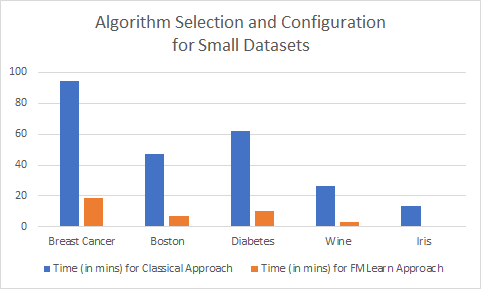
\includegraphics[width=15cm]{images/Small Datasets.png}
    \caption{Execution Time for Small Datasets as seen in Table \ref{table:1}}
    \label{fig:small_dataset}
\end{figure}

Hence, for a small dataset, the user saves an average of 48.79 minutes and about 92.24 minutes (for Breast-Cancer Dataset) in a best case scenario. Whereas, for a large dataset the user saves an average of 533.21 minutes and about 869.74 minutes (for Skin Segmentation Dataset) in a best case scenario. This amounts to about 86.72\% and 95.762\% (for small and large datasets respectively) of time spent waiting by the user, when the machine learning program performs algorithm selection and does hyper-parameter tuning to select the best parameters for the model. In a scenario where the user would want to re-optimize hyper parameters, re-training was required for only the best algorithm suggested by FMLearn. Under these circumstances, time saved on an average by the user was about 40.864 minutes for small datasets and 513.15 minutes for large datasets. These recommendations for best performing algorithms were consistent with the previously obtained results for the same data.

\begin{table}[H]
\centering 
\vspace*{+5pt}
 \begin{tabular}{ |p{1.8in}||p{1in}|p{0.7in}|p{1in}|p{0.8in}|  }
 \hline
 \multicolumn{5}{|c|}{Execution Time (in minutes) for Large Datasets} \\
 \hline
 Datasets & Optimize All Algorithms & FMLearn & Re-Optimise best algorithm & Saving in \%\\
 \hline
 Adult & 582.51 & 0.05 & 19.01 & 96.72 \\
 \hline
 MAGIC Gamma Telescope & 279.01 & 0.04 & 14.63 & 94.74 \\
  \hline
 Nursery & 256.42 &  0.04 & 15.47 & 93.95 \\
 \hline
 Skin Segmentation & 869.74 & 0.05 & 29.86 & 96.56 \\
 \hline
 Statlog-Shuttle & 678.37 & 0.04 & 21.35 & 96.84 \\
 \hline
 \hline
 \textbf{Average} & 533.21 & 0.044 & 20.06 & 95.762 \\
 \hline
\end{tabular}
\vspace*{+5pt}
\caption{Execution time when using GridSearch vs FMLearn for large datasets}
\label{table:2}
\end{table}
\vspace*{-10pt}

\begin{figure}[H]
    \centering
    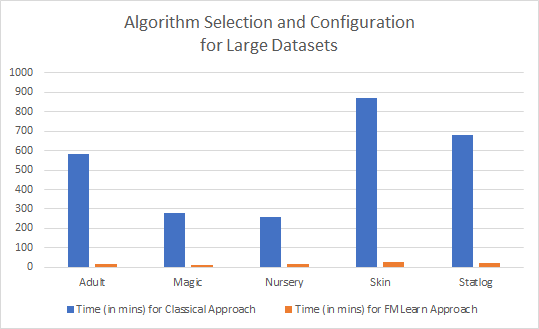
\includegraphics[width=15cm]{images/Large Datasets.png}
    \caption{Execution Time for Large Datasets as seen in Table \ref{table:2}}
    \label{fig:large_dataset}
\end{figure}

Figures \ref{fig:small_dataset} and \ref{fig:small_dataset} visually represent and compare the overall time consumed for traditional approach vs the approach involving FMLearn. From these figures we can see the advantages of using FMLearn over the traditional approach for algorithm selection or other AutoML libraries. FMLearn provides accurate and quick responses by making recommendation from a model created with historic performance data. Since, it is an ever growing and ever learning application, the recommendations made by FMLearn gets better over time. Time saved in percentage by using FMLearn for small and large datasets are represented in Figure \ref{fig:percentage_time_saved}.

\begin{figure}[H]
\centering
\begin{subfigure}{8cm}
  \centering
  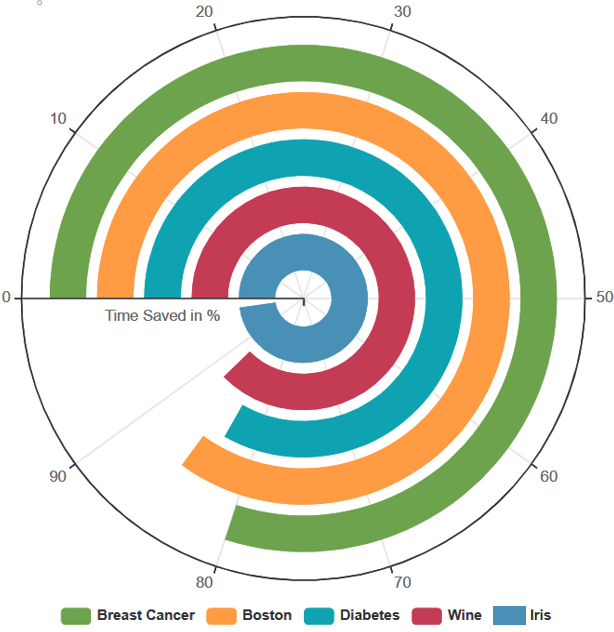
\includegraphics[width=\linewidth]{images/Percetnage Small Datasets.png}
  \caption{Small Dataset}
  \label{fig:small_dataset_time_Saved}
\end{subfigure}%
\begin{subfigure}{8cm}
  \centering
  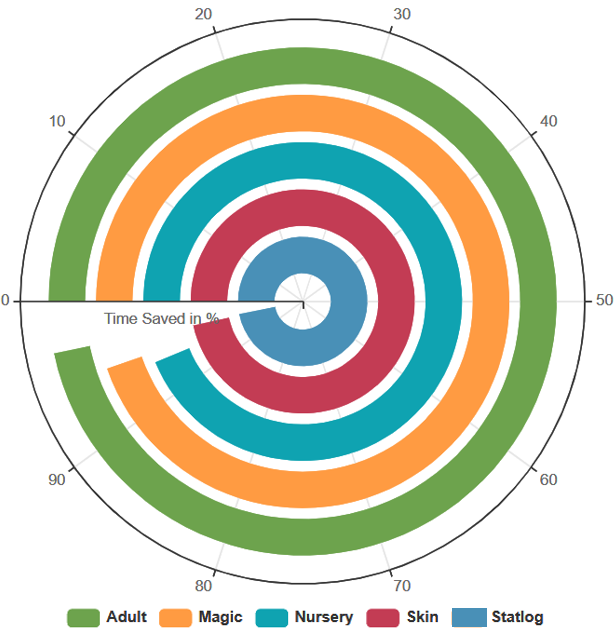
\includegraphics[width=\linewidth]{images/Percentage Large Datasets.png}
  \caption{Large Dataset}
  \label{fig:large_dataset_time_saved}
\end{subfigure}
\caption{Percentage of Time Saved}
\label{fig:percentage_time_saved}
\end{figure}


Upon considering the statistics obtained from the above results and using them in calculating the power consumption, we can see that the average power consumed for finding the best performing algorithm using the traditional approach for one of the small datasets is about 65.061W, but when using FMLearn the average power consumed is only about 10.629W which is about 86.718\% saving in the power used. In the case of large datasets, the average power consumed to find the best performing algorithm is about 710.946W, but when using FMLearn the average power consumed is only about 26.805W, which is about 95.762\% reduction in power used when compared to the traditional approach where FMLearn is not used.

\subsection*{Algorithm Recommendations}

Recommending the best algorithm falls into 3 different categories based on the closeness of the input dataset as explained in Section \ref{knn-model}, which can be categorised as follows:
\begin{itemize}
    \item Previously known dataset.
    \item Previously unknown dataset, which is similar to a known dataset.
    \item Previously unknown dataset, which is dissimilar to a known dataset.
\end{itemize}

The results discussed above are for previously known datasets. In the case of unknown but similar datasets, a the same experiment was conducted but with one modification, instead of using an known dataset, unknown yet, similar datasets was used. This similar datasets was obtained from a large dataset like the Statlog-Shuttle dataset. For example this dataset was taken and was broken down into small chunks of about 100k records, and these small subsets of data were used to get recommendations from FMLearn. Thought the meta-features of the dataset will vary, we can be confident that the changes in values will be not drastic as were obtained from the same parent dataset. In this case, the prediction of algorithm is accurate, but the hyper-parameters required re-optimisation to suite the new subset of the data. Whereas, in the case of an previously unseen dataset which is highly dissimilar to the datasets known to FMLearn, the model is able to predict the type machine learning problem the dataset belongs to, i.e, if it's a classification, regression, clustering, etc, but not the best algorithm for it, it instead recommends a set of algorithms which it thinks are the best in this case instead of recommending a single algorithm. In this case, the best performing algorithm is recommended by FMLearn about 60\% of the time. This set of algorithms are based on the closeness the previously known datasets.
\chapter{Conclusion}

From the evaluation of the concept of Federated Meta-Learning via implemented version of the application FMLearn, there is a clear improvement in the workflow of Algorithm Selection and Hyper-Parameter Optimisation. The algorithm recommendation system was specifically designed to replicate real work scenarios, thus facilitating the algorithm selection and configuration process. Though the application FMLearn is a prototype and a proof of concept for Federated Meta-Learning, the results proved that the concept and the application saves about 86.718\% of the time when compared to the traditional process of algorithm selection in the case of small datasets and about 95.762\% of time in the case of large datasets. Apart from saving time, the results also proved the reduced use of energy, thanks to the reduced amount of time consumed, 86.718\% and 95.762\% reduction for small and large datasets respectively. This reduction in energy and time will also save money and computational resources for developers.

The biggest contribution of FMLearn in the algorithm selection and configuration process is, elimination of the repetitive and time consuming nature of the task. Other major contributions can be attributed to the accurate nature of recommendations made and the ability of the system to grow overtime. As discussed in Section \ref{knn-model} and Section \ref{model-building}, FMLearn makes better predictions when it has more data to work with. The model rebuilding/retraining techniques used in the application makes it easier for FMLearn to make better predictions and improve user experience. 
\chapter{Limitations and Future Work}

FMLearn and Federated Meta-Learning opens up new avenues for research, the current implementation of FMLearn is a prototype, which just scratches the surface when compared to it's full potential.

\section*{Limitations}

The current implementation of FMLearn is limited to tabular datasets and feature‐based supervised machine learning algorithms. The limitation with respect to the use of tabular datasets is due to the fact that obtaining meta-features which describe different types of data like image, audio, video, etc., accurately are not available and is an area of intense research \citep{image-meta-data} \citep{image-meta-data-2} and there are no widely used tools available and developing such a tool is out of scope of this research. The restriction to use a feature-based supervised machine learning algorithms is that they are relatively less complex and have less number of hyper-parameters when compared to complex structures and thousands of hyper-parameters a neural network has, and implementing this was avoided due to the limitation in time.

\section*{Future Work}

The immediate future work concerning this project should be to move the client out of scikit-learn develop it as a stand alone library, this will enable wide spread use in the community which will result in the availability of vast variety of datasets. The increased availability will result in a better model thus improving the recommendations made my FMLearn. A more ambitious future work of this project could lead to research and implementation related to recommending complex neural networks or working with other forms of data source apart from tabular datasets.

\bibliographystyle{unsrtnat}
\bibliography{bibs/main}

\appendix
\renewcommand{\thechapter}{A\arabic{chapter}}
\chapter{Appendix}
\section{Code Availability}
All the code which is used for this paper is made available on GitHub:
\begin{itemize}
    \item The modified scikit-learn is available at: \newline \href{https://github.com/mukeshmk/scikit-learn}{https://github.com/mukeshmk/scikit-learn}
    \item The code for FMLearn application is available at: \newline \href{https://github.com/mukeshmk/fm-learn}{https://github.com/mukeshmk/fm-learn}
    \item The code used for the evaluation of the data is available at: \newline \href{https://github.com/mukeshmk/toy-datasets}{https://github.com/mukeshmk/toy-datasets}
\end{itemize}
The FMLearn application has also been deployed on heroku at \href{https://fmlearn.herokuapp.com/}{https://fmlearn.herokuapp.com/}. 

\textbf{NOTE:} this is just a API server, the website doesn't provide any functionality per-se.

\section{Meta-Features: Auto-Sklearn}
\label{meta-features-ask}

\textbf{TODO: Explain and represent in a better way}

\begin{lstlisting}
{
	"ClassEntropy": "0.9550393021523922"
    "SymbolsSum": "0.0"
    "SymbolsSTD": "0"
    "SymbolsMean": "0"
    "SymbolsMax": "0"
    "SymbolsMin": "0"
    "ClassProbabilitySTD": "0.12417582417582418"
    "ClassProbabilityMean": "0.5"
    "ClassProbabilityMax": "0.6241758241758242"
    "ClassProbabilityMin": "0.3758241758241758"
    "InverseDatasetRatio": "15.166666666666666"
    "DatasetRatio": "0.06593406593406594"
    "RatioNominalToNumerical": "0.0"
    "RatioNumericalToNominal": "0.0"
    "NumberOfCategoricalFeatures": "0"
    "NumberOfNumericFeatures": "30"
    "NumberOfMissingValues": "0.0"
    "NumberOfFeaturesWithMissingValues": "0.0"
    "NumberOfInstancesWithMissingValues": "0.0"
    "NumberOfFeatures": "30.0"
    "NumberOfClasses": "2.0"
    "NumberOfInstances": "455.0"
    "LogInverseDatasetRatio": "2.719100037288795"
    "LogDatasetRatio": "-2.7191000372887952"
    "PercentageOfMissingValues": "0.0"
    "PercentageOfFeaturesWithMissingValues": "0.0"
    "PercentageOfInstancesWithMissingValues": "0.0"
    "LogNumberOfFeatures": "3.4011973816621555"
    "LogNumberOfInstances": "6.12029741895095"
    "target_type": "binary"

}
\end{lstlisting}


\end{document}